\documentclass[12pt, a4paper, oneside]{report}

% ============================================================
% PACKAGES
% ============================================================
\usepackage[T1]{fontenc}
\usepackage[utf8]{inputenc}
\usepackage{amsmath, amssymb, amsfonts}
\usepackage{tabularx}
\usepackage{textcomp}           
\renewcommand{\rmdefault}{utm}   % Times New Roman
\usepackage{graphicx}           
\usepackage{float}              
\usepackage{array}              
\usepackage{caption}            
\captionsetup{labelsep=space}   
\usepackage[hidelinks]{hyperref}
\usepackage{setspace}            % For precise line spacing control
\newcommand{\degree}{$^\circ$}

% ============================================================
% PAGE GEOMETRY (1.5" left, 1" others)
% ============================================================
\setlength{\paperwidth}{210mm}
\setlength{\paperheight}{297mm}
\setlength{\oddsidemargin}{0.5in}    
\setlength{\evensidemargin}{0in}     
\setlength{\textwidth}{5.75in}       
\setlength{\topmargin}{0in}          
\setlength{\textheight}{9in}         
\setlength{\headheight}{0pt}
\setlength{\headsep}{0pt}
\setlength{\footskip}{0.5in}

% ============================================================
% LINE SPACING & PARAGRAPH
% ============================================================
\setstretch{1.3}  % ~1.5 line spacing for Times New Roman
\setlength{\parindent}{0pt}
\setlength{\parskip}{6pt} % Reduced from 18pt to fix excessive gap

% ============================================================
% HEADING FORMATS (Strictly matching PDF Guidelines)
% ============================================================
\makeatletter
\renewcommand{\chapter}{\if@openright\cleardoublepage\else\clearpage\fi
  \global\@topnum\z@
  \@afterindentfalse
  \secdef\@chapter\@schapter}
\def\@makechapterhead#1{%
  {\parindent \z@ \raggedright \normalfont\normalsize
    \bfseries \thechapter.\hspace{0.5em}\MakeUppercase{#1}\par\nobreak
    \vskip 12pt
  }}
\def\@makeschapterhead#1{%
  {\parindent \z@ \raggedright \normalfont\normalsize
    \bfseries \MakeUppercase{#1}\par\nobreak
    \vskip 12pt
  }}

\renewcommand\section{\@startsection{section}{1}{\z@}%
  {0pt}{10pt}{\normalfont\normalsize\bfseries}}
\renewcommand\subsection{\@startsection{subsection}{2}{\z@}%
  {0pt}{8pt}{\normalfont\normalsize\bfseries}}
\renewcommand\subsubsection{\@startsection{subsubsection}{3}{\z@}%
  {0pt}{6pt}{\normalfont\normalsize\bfseries}}

\renewcommand{\l@chapter}[2]{%
  \ifnum \c@tocdepth >\m@ne
    \addpenalty{-\@highpenalty}%
    \vskip 6pt
    \setlength\@tempdima{1.5em}%
    \begingroup
      \parindent \z@ \rightskip \@pnumwidth
      \parfillskip -\@pnumwidth
      \leavevmode \bfseries
      \advance\leftskip\@tempdima
      \hskip -\leftskip
      #1\nobreak
      \leaders\hbox{$\m@th \mkern \@dotsep mu\hbox{.}\mkern \@dotsep mu$}\hfill
      \nobreak\hb@xt@\@pnumwidth{\hss #2}\par
      \penalty\@highpenalty
    \endgroup
  \fi}
\makeatother

% ============================================================
% PAGE STYLE
% ============================================================
\pagestyle{plain} % Default page style (page numbers at bottom)

% ============================================================
% TOC / LOF / LOT FORMATTING
% ============================================================
\usepackage[titles]{tocloft}

\setlength{\cftbeforechapskip}{4pt}
\setlength{\cftbeforesecskip}{2pt}
\setlength{\cftbeforesubsecskip}{1pt}
\setlength{\cftbeforefigskip}{0pt}   
\setlength{\cftbeforetabskip}{0pt}   

\renewcommand{\cfttoctitlefont}{\normalsize\bfseries}
\renewcommand{\cftaftertoctitle}{\par\vskip 6pt}
\renewcommand{\cftloftitlefont}{\normalsize\bfseries}
\renewcommand{\cftafterloftitle}{\par\vskip 6pt} 
\renewcommand{\cftlottitlefont}{\normalsize\bfseries}
\renewcommand{\cftafterlottitle}{\par\vskip 6pt} 

\setlength{\cftbeforetoctitleskip}{0pt}
\setlength{\cftaftertoctitleskip}{0pt}
\setlength{\cftbeforeloftitleskip}{0pt}
\setlength{\cftafterloftitleskip}{0pt}
\setlength{\cftbeforelottitleskip}{0pt}
\setlength{\cftafterlottitleskip}{0pt}

\renewcommand{\contentsname}{TABLE OF CONTENTS}
\setcounter{tocdepth}{3}         
\setcounter{secnumdepth}{3}      

\renewcommand{\chaptername}{}
\makeatletter
\renewcommand{\@chapapp}{}
\makeatother

% ============================================================
% FIGURE AND TABLE NUMBERING
% ============================================================
\renewcommand{\thefigure}{\thechapter-\arabic{figure}}
\renewcommand{\thetable}{\thechapter-\arabic{table}}
\renewcommand{\theequation}{\thechapter-\arabic{equation}}

\renewcommand{\cftfigpresnum}{Figure }
\renewcommand{\cfttabpresnum}{Table }
\setlength{\cftfignumwidth}{5.5em}
\setlength{\cfttabnumwidth}{5em}

% ============================================================
% BIBLIOGRAPHY
% ============================================================
\renewcommand{\bibname}{REFERENCES}

\begin{document}

% =====================
% COVER & TITLE PAGES (No page numbers)
% =====================
\pagestyle{empty} % Temporarily disable page numbers
% Cover Page (First page - no page number)
\begin{titlepage}
\begin{center}
    \vspace*{0.5cm}

    
\includegraphics[width=3cm]{src/images/logo.png}\\
    \vspace{0.3cm}
    
    % --- University Info (12pt, Bold, Center) ---
    \textbf{\normalsize TRIBHUVAN UNIVERSITY}\\
    \textbf{\normalsize INSTITUTE OF ENGINEERING}\\
    \textbf{\normalsize THAPATHALI CAMPUS}\\
    
    \vfill
    
    % --- Report Type (12pt, Bold, Center) ---
    \textbf{\normalsize A Project Report}\\
    \textbf{\normalsize On}\\
    \vspace{0.5cm}
    
    % --- Project Title (14pt, Bold, Center) ---
    {\large \textbf{AI-Enhanced Prediction of El Niño and Its Impacts on South Asian Monsoon Precipitation and Temperature}}\\
    
    \vfill
    
    % --- Submitted By (12pt, Bold, Center) ---
    \textbf{\normalsize Submitted By:}\\
    
    \vspace{0.3cm}
    
    % --- Student Names (14pt, Center) ---
    \large 
    Biraj Adhikari (THA080BCT013)\\
    Raman Shrestha (THA080BCT031)\\
    Rojin Dhami (THA080BCT035)\\
    Sandeep Khadka (THA080BCT037)\\  
    
    \vfill
    
    % --- Submitted To (12pt, Bold, Center) ---
    \normalsize
    \textbf{\normalsize Submitted To:}\\
    
    \vspace{0.2cm}
    
    % --- Department Info (12pt, Center) ---
    \normalsize
    Department of Electronics and Computer Engineering\\
    Thapathali Campus\\
    Kathmandu, Nepal\\
    
    \vspace{0.5cm}
    
    % --- Date (12pt, Center) ---
    \normalsize
    August, 2026\\
    
\end{center}
\end{titlepage}
% Title Page (Second page - no page number)
\begin{titlepage}
\begin{center}
    \vspace*{0.5cm}
    
    
\includegraphics[width=3cm]{src/images/logo.png}\\
    \vspace{0.3cm}
    
    % --- 12pt, Bold, Center Justified ---
    \textbf{\normalsize TRIBHUVAN UNIVERSITY}\\
    \textbf{\normalsize INSTITUTE OF ENGINEERING}\\
    \textbf{\normalsize THAPATHALI CAMPUS}\\
    
    \vfill
    
    % --- 12pt, Bold, Center Justified ---
    \textbf{\normalsize A Project Report}\\
    \textbf{\normalsize On}\\
    
    \vspace{0.5cm}
    
    % --- Project Title (14pt, Bold, Center) ---
    {\large \textbf{AI-Enhanced Prediction of El Niño and Its Impacts on South Asian Monsoon Precipitation and Temperature}}\\
    
    \vfill
    
    % --- 12pt, Bold, Center Justified ---
    \textbf{\normalsize Submitted By:}\\
    
    \vspace{0.3cm}
    
    % --- 12pt, Center Justified (Strictly per PDF Title Page guideline) ---
    \normalsize
    Biraj Adhikari (THA080BCT013)\\
    Raman Shrestha (THA080BCT031)\\
    Rojin Dhami (THA080BCT035)\\
    Sandeep Khadka (THA080BCT037)\\  
    
    \vfill
    
    % --- 12pt, Bold, Center Justified ---
    \textbf{\normalsize Submitted To:}\\
    
    \vspace{0.2cm}
    
    % --- 12pt, Center Justified ---
    \normalsize
    Department of Electronics and Computer Engineering\\
    Thapathali Campus\\
    Kathmandu, Nepal\\
    
    \vspace{0.4cm}
    
    % --- 12pt, Center Justified ---
    \normalsize
    In partial fulfillment for the award of the Bachelor's Degree in\\
    Computer Engineering.\\
    
    \vspace{0.4cm}
    
    % --- 12pt, Bold, Center Justified ---
    \textbf{\normalsize Under the Supervision of}\\
    
    \vspace{0.2cm}
    
    % --- 12pt, Center Justified ---
    \normalsize
    Asst. Prof. Kobid Karkee\\
    
    \vspace{0.6cm}
    
    % --- 12pt, Center Justified ---
    \normalsize
    August, 2026\\
    
\end{center}
\end{titlepage}
\pagestyle{plain} % Restore page numbers for the rest of the document

% =====================
% FRONTMATTER (Starts Roman numbering: i, ii, iii...)
% =====================
\pagenumbering{roman}
\setcounter{page}{1} % Acknowledgement will be page 'i'
\chapter*{DECLARATION}
\addcontentsline{toc}{chapter}{DECLARATION}

We hereby declare that the report of the project entitled \textbf{``AI-Enhanced Prediction of El Niño and Its Impacts on South Asian Monsoon Precipitation and Temperature''} which is being submitted to the Department of Electronics and Computer Engineering, IOE, Thapathali Campus, in the partial fulfillment of the requirements for the award of the Degree of Bachelor of Engineering in Computer Engineering, is a bonafide report of the work carried out by us. The materials contained in this report have not been submitted to any University or Institution for the award of any degree and we are the only author of this complete work and no sources other than the listed here have been used in this work.

\vspace{2cm}

% --- Perfectly Aligned Signature Block ---
\noindent
\begin{tabular}{@{}p{6.5cm}@{\hspace{1cm}}l@{}}
    Biraj Adhikari (THA080BCT013) & \rule{5cm}{0.6pt} \\[0.5cm]
    Raman Shrestha (THA080BCT031) & \rule{5cm}{0.6pt} \\[0.5cm]
    Rojin Dhami (THA080BCT035) & \rule{5cm}{0.6pt} \\[0.5cm]
    Sandeep Khadka (THA080BCT037) & \rule{5cm}{0.6pt}
\end{tabular}

\vspace{1cm}

\noindent Date: August, 2026
\chapter*{CERTIFICATE OF APPROVAL}
\addcontentsline{toc}{chapter}{CERTIFICATE OF APPROVAL}

The undersigned certify that they have read and recommend to the Department of Electronics and Computer Engineering, IOE, Thapathali Campus, the minor project work entitled \textbf{``AI-Enhanced Prediction of El Niño and Its Impacts on South Asian Monsoon Precipitation and Temperature''}, submitted by Biraj Adhikari, Raman Shrestha, Rojin Dhami, and Sandeep Khadka in partial fulfillment of the requirements for the Bachelor's Degree in Computer Engineering. The project was carried out under supervision and within the prescribed time frame.

\vspace{0.3cm}

\noindent We found the students to be hardworking, skilled, and capable of undertaking related work in their field of study. Hence, we recommend the project for partial fulfillment of the requirements for the Bachelor's Degree in Computer Engineering.

\vspace{0.6cm}

% --- Supervisor ---
\noindent \rule{5.5cm}{0.4pt} \\[0.08cm]
Project Supervisor \\[0.03cm]
Asst. Prof. Kobid Karkee \\
Department of Electronics and Computer Engineering, Thapathali Campus

\vspace{0.5cm}

% --- External Examiner ---
\noindent \rule{5.5cm}{0.4pt} \\[0.08cm]
External Examiner \\[0.03cm]


\vspace{0.5cm}

% --- Project Co-ordinator ---
\noindent \rule{5.5cm}{0.4pt} \\[0.08cm]
Project Co-ordinator \\[0.03cm]
Asst. Prof. Anup Shrestha \\
Department of Electronics and Computer Engineering, Thapathali Campus

\vspace{0.5cm}

% --- Head of Department ---
\noindent \rule{5.5cm}{0.4pt} \\[0.08cm]
Head of the Department \\[0.03cm]
Mr. Umesh Kanta Ghimire \\
Department of Electronics and Computer Engineering, Thapathali Campus

\vspace{0.3cm}

\noindent Date: August, 2026
\input{report/src/frontmatter/copyright}
\chapter*{ACKNOWLEDGEMENT}
\addcontentsline{toc}{chapter}{ACKNOWLEDGEMENT}

\bigskip

We express our sincere gratitude to the Department of Electronics and Computer Engineering, Thapathali Campus, for providing us the opportunity to undertake this minor project on ``AI-Enhanced Prediction of El Ni\~{n}o and its Regional Climatic Impacts''

We are deeply thankful to our project supervisor Asst. Prof. Kobid Karkee for his invaluable guidance, constructive feedback, and continuous encouragement throughout the proposal preparation and planned project work. His expertise in machine learning and climate modeling has been instrumental in shaping our approach and in helping us anticipate and address technical challenges.

We also appreciate the support from our faculty members and peers who provided insightful suggestions during discussions on topic selection, literature review, and methodology design. Special thanks go to the open-source community, especially the providers of the ERA5 and ORAS5 datasets, for making state-of-the-art climate reanalysis data easily accessible to students and researchers.

Finally, we are grateful to our families and friends for their patience, motivation, and consistent support during the extended hours of study, experimentation, and documentation required for this proposal.

\vspace{2em}
\noindent Biraj Adhikari (THA080BCT013) \\
Raman Shrestha (THA080BCT031) \\
Rojin Dhami (THA080BCT035) \\
Sandeep Khadka (THA080BCT037)

\chapter*{ABSTRACT}
\addcontentsline{toc}{chapter}{ABSTRACT}
\bigskip

El Ni\~{n}o events can substantially influence the South Asian monsoon, creating important implications for agriculture, water resources, and disaster preparedness. This project develops a deep learning framework for forecasting the El Ni\~{n}o--Southern Oscillation (ENSO) state 3 to 6 months in advance and assessing its potential impacts on South Asian precipitation and temperature. The framework uses climate data from 1980 to 2025, incorporating publicly available reanalysis datasets, including ERA5 and ORAS5, together with established ENSO indices. A hybrid CNN-TCN architecture is employed, where the CNN component extracts spatial patterns from monthly sea surface temperature (SST) fields, while the TCN component captures their temporal evolution over the 12-month input sequence. The primary prediction target is the Ni\~{n}o 3.4 index, which is used as an indicator of the ENSO state. Evaluated using a 5-seed ensemble, the model achieves a mean 3-month lead Ni\~{n}o 3.4 RMSE of 0.51\degree C and a Pearson correlation of 0.92. The predicted ENSO state is subsequently used to derive an ENSO-based assessment of South Asian precipitation and temperature anomalies. The resulting pipeline provides a deterministic ENSO-based outlook and corresponding impact assessment for the 2026 June--September monsoon season, demonstrating the potential of deep learning-based ENSO forecasting to support climate-risk assessment, disaster preparedness, and resource management in South Asia.

\vspace{1em}
\noindent\textit{\textbf{Keywords}}: \textit{CNN-TCN, Deep Learning, El Ni\~{n}o, ENSO, Ni\~{n}o 3.4, Sea Surface Temperature}.

\clearpage

% TOC (1.0 line spacing per guideline for extensive lists)
\begingroup
  \setstretch{1.0}
  \tableofcontents
\endgroup
\clearpage

% LIST OF FIGURES with proper spacing
\begingroup
  \setstretch{1.0}                    % Single line spacing (per guidelines)
  \setlength{\parskip}{0pt}           % Remove paragraph spacing
  \setlength{\cftbeforefigskip}{0pt}  % Remove space between figure entries
  \raggedbottom                       % Prevent vertical stretching
  \addcontentsline{toc}{chapter}{LIST OF FIGURES}
  \renewcommand{\listfigurename}{LIST OF FIGURES}
  \listoffigures
\endgroup
\clearpage

% LIST OF TABLES (Spacing Fixed)
\begingroup
  \setstretch{1.0}
  \setlength{\parskip}{0pt}
  \setlength{\cftbeforetabskip}{3pt} % Uniform 3pt spacing between tables
  \raggedbottom % Prevents stretching
  \addcontentsline{toc}{chapter}{LIST OF TABLES}
  \renewcommand{\listtablename}{LIST OF TABLES}
  \listoftables
\endgroup
\clearpage

% LIST OF ABBREVIATIONS
\chapter*{LIST OF ABBREVIATIONS}
\addcontentsline{toc}{chapter}{LIST OF ABBREVIATIONS}

\bigskip

\begin{tabbing}
\hspace*{3cm}\=\kill
\textbf{ACC} \> Anomaly Correlation Coefficient \\
\textbf{AI} \> Artificial Intelligence \\
\textbf{CMIP6} \> Coupled Model Intercomparison Project Phase 6 \\
\textbf{CNN-TCN} \> Convolutional Neural Network -- Temporal Convolutional Network \\
\textbf{CORDEX} \> Coordinated Regional Climate Downscaling Experiment \\
\textbf{DESN} \> Deep Echo State Network \\
\textbf{DL} \> Deep Learning \\
\textbf{ECMWF} \> European Centre for Medium-Range Weather Forecasts \\
\textbf{ENSO} \> El Ni\~{n}o-Southern Oscillation \\
\textbf{ESN} \> Echo State Network \\
\textbf{GCM} \> General Circulation Model \\
\textbf{GODAS} \> Global Ocean Data Assimilation System \\
\textbf{GPU} \> Graphics Processing Unit \\
\textbf{JJAS} \> June-July-August-September \\
\textbf{LSTM} \> Long Short-Term Memory \\
\textbf{MAE} \> Mean Absolute Error \\
\textbf{MEI} \> Multivariate ENSO Index \\
\textbf{MIFS} \> Mutual Information Feature Selection \\
\textbf{ML} \> Machine Learning \\
\textbf{NOAA} \> National Oceanic and Atmospheric Administration \\
\textbf{ORAS5} \> Ocean Reanalysis System 5 \\
\textbf{RF} \> Random Forest \\
\textbf{RMSE} \> Root Mean Square Error \\
\textbf{RNN} \> Recurrent Neural Network \\
\textbf{ResNet} \> Residual Network \\
\textbf{SLP} \> Sea Level Pressure \\
\textbf{SST} \> Sea Surface Temperature \\
\textbf{XGBoost} \> Extreme Gradient Boosting \\
\end{tabbing}

\clearpage

% =====================
% MAINMATTER (Starts Arabic numbering: 1, 2, 3...)
% =====================
\pagenumbering{arabic}
\setcounter{page}{1}

\chapter{INTRODUCTION}

\section{Background}

The El Ni\~{n}o-Southern Oscillation (ENSO) is the dominant mode of interannual climate variability, influencing weather patterns worldwide through coupled ocean-atmosphere interactions in the tropical Pacific \cite{ham2019deep}. ENSO cycles between warm (El Ni\~{n}o) and cool (La Ni\~{n}a) phases, driven primarily by anomalies in Sea Surface Temperature (SST) across the equatorial Pacific Ocean. These events have far-reaching teleconnections that affect precipitation, temperature, and extreme weather events across multiple continents.

Furthermore, anthropogenic climate change is increasingly modulating ENSO dynamics. Recent climatological studies indicate a trend toward more frequent and intense extreme ENSO events, including a higher occurrence of Central Pacific (Modoki) El Ni\~{n}os and ``Super El Ni\~{n}os'' \cite{cai2015continued}. This non-stationarity in the background state of the tropical Pacific complicates the physical mechanisms driving ENSO, thereby exacerbating the ``spring predictability barrier'' and challenging the skill of traditional dynamical models.

South Asia, where the Indian Summer Monsoon provides over 70\% of annual rainfall, is highly vulnerable to ENSO-induced climate anomalies \cite{ye2024resonet}. El Ni\~{n}o events are associated with weakened monsoon circulation, leading to droughts in the Indian subcontinent, while La Ni\~{n}a events often intensify monsoon rainfall \cite{mahesh2024physics}. Climate outlooks indicate the possibility of ENSO-related anomalies during 2026, highlighting the importance of improved forecasting systems.

Nepal, situated in the central Himalayas, is particularly susceptible to these teleconnections due to its fragile topography and heavy reliance on monsoon-dependent agriculture and hydropower. ENSO phases significantly dictate the spatial and temporal distribution of precipitation across Nepal's diverse elevational gradients. During El Ni\~{n}o years, Nepal frequently experiences below-normal monsoon rainfall and delayed monsoon onsets, which critically deplete soil moisture, reduce hydropower generation capacity, and trigger winter and spring droughts. Conversely, La Ni\~{n}a phases are often associated with above-normal rainfall, increasing the risk of catastrophic flooding and landslides in the steep river basins \cite{shrestha2021enso}.

Traditional dynamical climate models, such as General Circulation Models (GCMs), provide seasonal ENSO forecasts but face limitations in prediction skill beyond 6--9 months due to the ``spring predictability barrier'' \cite{dijkstra2019deep}. Recent advances in deep learning have demonstrated superior forecasting skill at longer lead times (12--22 months) by extracting complex spatiotemporal patterns from vast reanalysis archives \cite{ham2019deep, mahesh2024physics}. These data-driven approaches leverage Convolutional Neural Networks (CNNs) and Long Short-Term Memory (LSTM) networks to capture nonlinear dynamics that traditional statistical methods and dynamical models struggle to represent.

\section{Motivation}
The motivation for this project stems from three critical factors:

\begin{itemize}
    \item \textbf{Imminent Climate Risk:} The 2026 El Ni\~{n}o poses significant risks to South Asia's agriculture, water resources, and disaster management infrastructure. Early and accurate prediction enables proactive mitigation strategies.
    
    \item \textbf{Limitations of Existing Models:} While dynamical models provide reasonable short-term ENSO forecasts, their skill degrades significantly beyond one season. Deep learning models have shown promise in extending this predictability horizon but are often not tailored to regional impact assessment.
    
    \item \textbf{Need for Actionable Regional Forecasts:} Most existing ENSO prediction systems focus on the Ni\~{n}o 3.4 index alone without providing spatially resolved impact assessments for vulnerable regions. There is a critical gap between global ENSO state prediction and localized climate impact forecasting.
\end{itemize}

\section{Problem Statement}
Despite significant progress in ENSO forecasting using deep 
learning, existing approaches face key limitations:

\begin{itemize}
    \item Most models predict only the Ni\~{n}o 3.4 index 
    without translating predictions into regional climate 
    impacts, limiting their practical utility for 
    disaster preparedness and agricultural planning.
    
    \item No unified deep learning framework currently exists 
    that couples ENSO state forecasting with deterministic 
    regional impact assessment specifically for South Asian 
    precipitation and temperature anomalies.
\end{itemize}

This project addresses these gaps by developing a multi-task 
CNN-TCN framework that forecasts ENSO state at 6 month lead times 
and simultaneously produces deterministic precipitation and 
temperature anomaly maps over South Asia.

\section{Objectives}
The primary objectives of this project are as follows:
\begin{itemize}
    \item To develop a CNN-TCN model to forecast the 
    Ni\~{n}o 3.4 index at a 6-month lead time using 
    ERA5 and ORAS5 reanalysis data spanning 1980--2025.
    
    \item To develop a coupled impact assessment module 
    that produces deterministic forecasts of 
    June--July--August--September precipitation 
    and temperature anomalies over South Asia based on 
    the predicted Ni\~{n}o 3.4 index.
\end{itemize}

\section{Scope and Limitations}

\subsection{Scope}
\begin{itemize}
    \item The system will forecast ENSO states using the Ni\~{n}o 3.4 index at lead times of 6 months.
    \item Regional impact assessment will cover the South Asian domain (5$^{\circ}$N--40$^{\circ}$N, 60$^{\circ}$E--100$^{\circ}$E).
    \item The model will be trained on publicly available datasets including ERA5 and ORAS5.
    \item The final deliverable will include a functional forecasting pipeline implemented in Python.
\end{itemize}

\subsection{Limitations}
\begin{itemize}
    \item The model is trained on historical data and may not capture unprecedented climate dynamics.
    \item The system does not account for other climate drivers (e.g., Indian Ocean Dipole, Arctic Oscillation) that may modulate ENSO impacts.
    \item Real-time operational deployment is beyond the scope of this project.
\end{itemize}

\section{Project Applications}
\begin{itemize}
    \item \textbf{Agricultural Planning:} The system provides early warning for monsoon deficiency or excess rainfall, enabling farmers and agricultural agencies to guide crop planning and irrigation management.

    \item \textbf{Disaster Preparedness:} The framework identifies regions at elevated flood or drought risk, allowing disaster management authorities to undertake proactive resource allocation.

    \item \textbf{Water Resource Management:} Seasonal reservoir operation planning is supported through deterministic precipitation forecasts generated by this system.

    \item \textbf{Climate Research:} The project contributes to the broader scientific understanding of ENSO teleconnections and advances AI-based climate prediction methodologies.
\end{itemize}

\chapter{LITERATURE REVIEW}

\section{ENSO Prediction: From Dynamical Models to Deep Learning}

The prediction of ENSO has been a central challenge in climate science for over four decades. Early approaches relied on linear statistical models and dynamical ocean-atmosphere coupled models \cite{dijkstra2019deep}. While dynamical models based on General Circulation Models (GCMs) can capture the fundamental physics of ENSO, their predictive skill drops sharply beyond 6--9 months due to the well-documented ``spring predictability barrier,'' where forecast initialization errors grow rapidly during boreal spring \cite{mahesh2024physics}.

The advent of machine learning and deep learning has opened new avenues for ENSO prediction. Unlike dynamical models that solve physical equations numerically, data-driven approaches learn complex nonlinear mappings directly from observational data, potentially capturing dynamics that are poorly represented in physical models.

\section{Deep Learning Approaches for ENSO Forecasting}

\subsection{CNN-Based Multi-Year ENSO Forecasting}

Ham et al. \cite{ham2019deep} demonstrated a breakthrough in ENSO prediction by applying transfer learning with CNNs to forecast the Ni\~{n}o 3.4 index at lead times exceeding 18 months. Their approach addressed the fundamental challenge of limited observational data by pre-training the CNN on historical simulations from CMIP5 climate models and fine-tuning on reanalysis data (1871--1973 for training, 1984--2017 for testing). The CNN architecture processes monthly maps of SST, ocean heat content (upper 300m), and sea level pressure as multi-channel inputs, producing Ni\~{n}o 3.4 index predictions at various lead times.

The model achieved an all-season correlation skill of 0.65 at 17-month lead time, substantially outperforming both dynamical models and conventional statistical methods. Importantly, the CNN successfully predicted the onset and amplitude of El Ni\~{n}o events that traditional models missed. Gradient-based saliency analysis revealed that the network learned physically meaningful precursor patterns, including subsurface heat content anomalies in the western Pacific that serve as recharged energy for subsequent El Ni\~{n}o development. However, the model showed reduced skill for La Ni\~{n}a events and lacked uncertainty quantification.

\subsection{Autoencoder-LSTM Hybrid Architecture}

Dijkstra et al. \cite{dijkstra2019deep} proposed a hybrid deep learning architecture combining autoencoders with LSTM networks for ENSO forecasting. Their approach first employs a convolutional autoencoder to compress high-dimensional SST fields into a low-dimensional latent representation, effectively performing nonlinear dimensionality reduction. The temporal evolution of these latent features is then modeled using an LSTM network, which captures the sequential dependencies inherent in ENSO dynamics.

The autoencoder-LSTM framework was trained on SODA reanalysis data and evaluated against persistence forecasts and linear inverse models. The model demonstrated competitive skill at lead times of 6--12 months, with the autoencoder successfully capturing the dominant spatial patterns of ENSO variability (comparable to traditional EOF analysis but with nonlinear generalization). The LSTM component effectively learned the oscillatory nature of ENSO transitions between warm and cool phases. The authors noted that the latent space representation provided physical interpretability, with different latent dimensions corresponding to recognizable ENSO precursor patterns.

\subsection{Physics-Guided Deep Echo State Networks}

Mahesh et al. \cite{mahesh2024physics} introduced a physics-guided Deep Echo State Network (DESN) approach to enhance ENSO predictability limits. Echo State Networks (ESNs) are a variant of recurrent neural networks where the recurrent layer (reservoir) has fixed random weights, and only the output layer is trained. This architecture offers computational efficiency and avoids the vanishing gradient problem that plagues conventional RNNs during training.

The key innovation in their work is the incorporation of physics-based constraints into the ESN framework. Specifically, they embed known ENSO dynamics, such as the recharge-discharge oscillator mechanism and delayed oscillator theory, as structural priors in the reservoir connectivity. The physics-guided DESN achieved prediction skill comparable to deep learning baselines (correlation $>$ 0.5 at 18-month lead) while requiring significantly fewer trainable parameters and providing enhanced interpretability.

The model was trained on ERA5 reanalysis data with SST, thermocline depth, and zonal wind stress as inputs. A notable advantage is the model's ability to overcome the spring predictability barrier more effectively than purely data-driven approaches, attributed to the physics constraints preventing the model from learning spurious correlations that break down during spring transitions.

\subsection{ResoNet: Robust and Explainable ENSO Forecasting}

Ye et al. \cite{ye2024resonet} developed ResoNet, a hybrid deep learning framework combining Residual Network (ResNet) architecture with physical ocean dynamics for robust and explainable ENSO forecasting. The model integrates residual learning blocks that capture multi-scale spatiotemporal features from SST, ocean heat content, and wind stress fields. A key contribution is the attention mechanism that identifies physically meaningful precursor regions.

ResoNet achieved state-of-the-art performance with correlation skills exceeding 0.7 at 12-month lead time and maintained useful skill ($>$ 0.5) beyond 18 months. The explainability module generates spatial attribution maps highlighting the oceanic regions most influential for each prediction, enhancing trust in the model's outputs. The model demonstrated particular strength in predicting the diversity of El Ni\~{n}o events (Eastern Pacific vs. Central Pacific types), a capability lacking in many earlier deep learning approaches. The framework also incorporated ensemble prediction to provide uncertainty estimates, generating probabilistic forecasts rather than single deterministic predictions.

\section{Machine Learning for Regional Climate Impact Assessment}

\subsection{ENSO-Driven Weather Pattern Prediction}

Dutta et al. \cite{dutta2024seasonal} investigated the application of machine learning for predicting seasonal weather patterns from ENSO indices, bridging the gap between large-scale ENSO state prediction and regional climate impacts. Their study employed Random Forest, Gradient Boosting, and Support Vector Machine classifiers to predict seasonal precipitation and temperature categories (below normal, normal, above normal) conditioned on multivariate ENSO indicators including Ni\~{n}o 3.4, Southern Oscillation Index (SOI), and the Multivariate ENSO Index (MEI).

The results demonstrated that ensemble machine learning methods, particularly XGBoost and Random Forest, achieved classification accuracies of 70--82\% for seasonal precipitation categories when ENSO indices from 2--3 months prior were used as predictors. Feature importance analysis revealed that the combination of Ni\~{n}o 3.4 amplitude and rate of change provided the strongest predictive signal for South Asian monsoon anomalies. However, the study was limited to categorical predictions and did not provide spatially resolved forecasts.

\section{Comparison of Existing Approaches}

Table \ref{tab:lit_comparison} summarizes the key characteristics and performance metrics of the reviewed ENSO forecasting approaches.

\begin{table}[ht]
\centering
\caption{Comparison of Deep Learning Approaches for ENSO Forecasting}
\label{tab:lit_comparison}
\small
\begin{tabular}{|l|l|c|c|c|}
\hline
\textbf{Study} & \textbf{Method} & \textbf{Max Lead} & \textbf{Corr.} & \textbf{Uncert.} \\
\hline
Ham et al. \cite{ham2019deep} & CNN + Transfer Learning & 17 mo. & 0.65 & No \\
\hline
Dijkstra et al. \cite{dijkstra2019deep} & Autoencoder + LSTM & 12 mo. & 0.60 & No \\
\hline
Mahesh et al. \cite{mahesh2024physics} & Physics-guided DESN & 18 mo. & 0.50 & No \\
\hline
Ye et al. \cite{ye2024resonet} & ResoNet (ResNet + Physics) & 18 mo. & 0.70 & Yes \\
\hline
Dutta et al. \cite{dutta2024seasonal} & XGBoost/RF Classification & 3 mo. & 0.82 & No \\
\hline
\end{tabular}
\end{table}



\chapter{REQUIREMENT ANALYSIS}

This chapter enumerates and describes the hardware, software, and data components required for the successful execution of the ENSO forecasting project. It also evaluates the technical, economic, time, and operational feasibility of the proposed system.

\section{Project Requirements}

The development of a deep learning framework for ENSO forecasting and regional climate impact assessment requires specific computational resources, software tools, and high-dimensional climate datasets. These requirements are detailed below.

\subsection{Hardware Requirements}

While the initial data preprocessing and baseline model development can be performed on standard local machines, the training of the Convolutional Neural Network--Temporal Convolutional Network (CNN-TCN) architecture requires significant computational power. 
\begin{itemize}
    \item \textbf{Local Development Machine:} A standard laptop or desktop computer with at least 16 GB of RAM and a multi-core processor for code development, data inspection, and lightweight baseline testing (e.g., XGBoost).
    \item \textbf{Cloud GPU Computing:} Access to high-performance cloud GPUs (such as NVIDIA Tesla V100 or A100 via Google Colab Pro or AWS EC2) is strictly required. Training deep learning models on 45 years of 2\degree $\times$ 2\degree spatiotemporal climate data involves millions of parameters and large batch processing, which exceeds the capacity of standard consumer hardware.
    \item \textbf{Storage:} Approximately 500 GB to 1 TB of storage (local or cloud-based) is required to store the raw and processed NetCDF and Zarr files for the ERA5 and ORAS5 datasets.
\end{itemize}

\subsection{Software Requirements}

The project relies entirely on open-source software and standard scientific computing libraries. The core software stack includes:
\begin{itemize}
    \item \textbf{Programming Language:} Python 3.8 or higher, chosen for its extensive ecosystem in machine learning and data science.
    \item \textbf{Deep Learning Frameworks:} PyTorch or TensorFlow for building, training, and evaluating the CNN-TCN hybrid architecture.
    \item \textbf{Data Processing and Analysis:} Xarray for handling multi-dimensional climate arrays (NetCDF/Zarr), Pandas and NumPy for data manipulation, and Scikit-learn for feature selection (MIFS) and baseline modeling.
    \item \textbf{API and Version Control:} The Copernicus Climate Data Store (CDS) API for automated data fetching, and Git/GitHub for version control and collaborative code management.
    \item \textbf{Documentation:} \LaTeX{} (via Overleaf) for compiling the final report according to IOE formatting guidelines.
\end{itemize}

\subsection{Data Requirements}

The model requires high-quality, long-term historical climate data to capture interannual variability. The specific datasets include:
\begin{itemize}
    \item \textbf{ERA5 Reanalysis Data:} Monthly-mean Sea Surface Temperature (SST), 2-meter temperature, and precipitation data from the Copernicus Climate Data Store.
    \item \textbf{ORAS5 Ocean Reanalysis:} Subsurface ocean variables (temperature and salinity) accessed via the ARCO Zarr store to provide depth-related ENSO precursor signals.
    \item \textbf{NOAA Ni\~{n}o Indices:} Official historical Ni\~{n}o 3.4 indices used as the ground truth for validating the model's predictive accuracy.
\end{itemize}

\section{Feasibility Study}

A comprehensive feasibility analysis was conducted to ensure that the project objectives can be realistically achieved within the given constraints.

\subsection{Technical Feasibility}

The project is technically feasible given the availability of all required datasets through public repositories (ECMWF CDS, NOAA, ESGF). The Convolutional Neural Network--Temporal Convolutional Network (CNN-TCN) architecture is well-supported in PyTorch, and the 45-year dataset (1980--2025) provides sufficient temporal coverage for robust model training. The six-stage pipeline (data ingestion, preprocessing, feature engineering, MIFS feature selection, model development, and forecasting) is modular and implementable within the team's existing Python and machine learning skill set.

\subsection{Economic Feasibility}

The project incurs near-zero data and software costs, as all datasets and development tools are freely available. The primary expenditure is cloud compute (Google Colab Pro) for CNN-TCN training on ERA5 and ORAS5 reanalysis fields. The total estimated budget of NPR~10,500 is well within the means of a student project group, with no specialized hardware procurement required.

\subsection{Time Feasibility}

Based on the project schedule spanning June 1 to September 7, 2025 (approximately 14 weeks), the timeline is realistic and well-structured. The work begins with literature review, data collection, and preprocessing in the first four weeks, followed by feature engineering, MIFS feature selection, and parallel development of the XGBoost baseline and CNN-TCN model through mid-August. Model training, hyperparameter tuning, forecast generation, and evaluation are conducted in the final weeks, with documentation and report writing running concurrently from mid-August through project completion. Tasks are sequenced with deliberate overlaps (for instance, XGBoost baseline and CNN-TCN development proceed in parallel) to maximize efficiency within the 14-week window.

\subsection{Operational Feasibility}

The project delivers a self-contained Python-based forecasting pipeline publishable as an open-source GitHub repository. The modular architecture ensures each stage can be independently tested and debugged. All four team members bring complementary skills in machine learning, data preprocessing, and climate data handling, ensuring balanced workload distribution. The final outputs (ENSO state forecasts and deterministic South Asian precipitation and temperature anomaly maps for JJAS 2026) are directly interpretable and actionable for the target academic audience.
\chapter{SYSTEM ARCHITECTURE AND METHODOLOGY}
\label{chap:methodology}

\section{System Overview}

The system follows an eight-stage pipeline architecture:
\begin{enumerate}
    \item Data ingestion
    \item Data preprocessing
    \item Feature engineering
    \item Feature selection
    \item Baseline model development
    \item Deep learning model training
    \item Model validation
    \item 2026 ENSO forecasting
\end{enumerate}
The framework ingests multi-variable climate reanalysis data and produces ENSO state predictions at 6-month lead times along with regional precipitation and temperature anomaly forecasts for South Asia.

\section{System Architecture}

\begin{figure}[H]
    \centering
    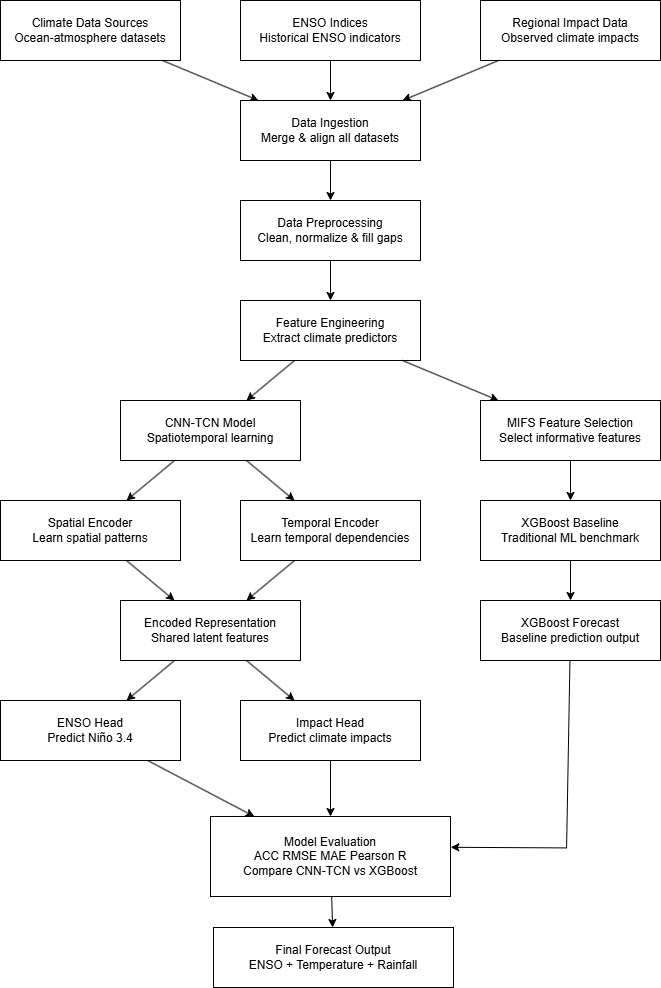
\includegraphics[width=0.85\textwidth]{src/images/system_architecture.png}
    \captionsetup{justification=centering}
    \caption{System Architecture of the project}
    \label{fig:system_architecture}
\end{figure}

The system architecture comprises eight sequential stages: (1) \textbf{Data Ingestion}, where multi-variable climate reanalysis datasets (ERA5, ORAS5, NOAA) are acquired from public repositories; (2) \textbf{Data Preprocessing}, which includes spatial standardization to a uniform 2\degree$\times$2\degree\ grid, temporal alignment to the common period 1980--2025, climatological anomaly computation, and z-score normalization; (3) \textbf{Feature Engineering}, where 12-month sliding window input tensors of shape $(12 \times 30 \times 100 \times 6)$ are constructed from the six spatial fields; (4) \textbf{Feature Selection}, applying Mutual Information Feature Selection (MIFS) for the XGBoost baseline; (5) \textbf{Baseline Model Development}, comprising the XGBoost baseline; (6) \textbf{Deep Learning Model Training}, comprising the CNN-TCN deep learning model; (7) \textbf{Model Validation}, where the models are evaluated; and (8) \textbf{Forecasting}, where the trained model generates 3-month and 6-month lead Ni\~{n}o 3.4 index predictions and regional South Asian precipitation and temperature anomaly forecasts.

\begin{figure}[H]
    \raggedleft
    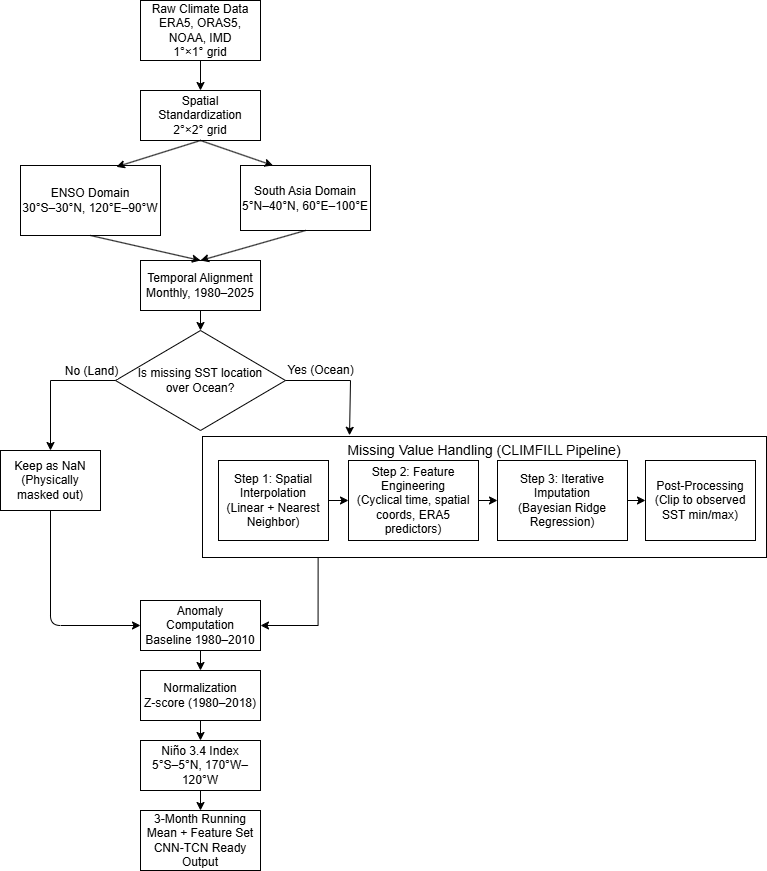
\includegraphics[width=0.85\textwidth]{src/images/data_preprocess.png}
    \captionsetup{justification=centering}
    \caption{Data Preprocessing Pipeline}
    \label{fig:data_preprocess}
\end{figure}

The data preprocessing pipeline (Figure \ref{fig:data_preprocess}) transforms raw climate reanalysis fields into analysis-ready inputs through four sequential operations: spatial standardization via area-weighted block averaging to a 2\degree$\times$2\degree\ grid, temporal alignment ensuring all variables share the 1980--2025 monthly time axis, climatological anomaly computation by subtracting the long-term monthly mean, and z-score normalization to scale all fields to have a mean of 0 and a standard deviation of 1 for stable model training.

\section{Data Sources}

The project utilizes the following publicly available datasets:

\subsection{Oceanic \& Atmospheric Reanalysis}
\begin{itemize}
    \item \textbf{ERA5 Reanalysis (ECMWF):} Monthly SST, sea level pressure (SLP), 2m temperature (T2M), and wind stress fields at 1\degree$\times$1\degree\ resolution (1950--2025).
    \item \textbf{ORAS5 (ECMWF):} Ocean heat content and subsurface temperature profiles for the tropical Pacific.
\end{itemize}

\subsection{ENSO Indices}
\begin{itemize}
    \item \textbf{Ni\~{n}o 3.4 Index (NOAA):} Monthly SST anomaly in the Ni\~{n}o 3.4 region (5\degree N--5\degree S, 170\degree W--120\degree W), serving as the primary ENSO indicator (1871--present).
\end{itemize}

\section{Workflow}

The project follows an eight-step pipeline: data ingestion, data preprocessing, feature engineering, feature selection, baseline model development, deep learning model training, model validation, and 2026 forecasting. The data-facing steps of this pipeline are described below; the feature selection strategy, the baseline model, and the deep learning model are each developed in dedicated sections (Sections~\ref{sec:feature-selection}--\ref{sec:cnn-tcn}) given the depth of methodological detail each requires.

\subsection{Data Ingestion}
All datasets are aggregated, resampled to a consistent monthly 2\degree$\times$2\degree\ grid, and aligned to the common period 1980--2025. Data quality checks and gap-filling procedures are applied to ensure temporal continuity.

\subsection{Data Preprocessing}

The raw climate datasets ingested from ERA5, ORAS5, and NOAA undergo the following preprocessing steps prior to feature engineering:

\noindent\textbullet\ \textbf{Spatial Standardization}\\
All datasets are ingested at their native 1\degree\ latitude $\times$ 1\degree\ longitude spatial resolution. A 1\degree\ latitude $\times$ 1\degree\ longitude grid cell covers approximately 111 km (along latitude) $\times$ 111 km (along longitude) at the equator, representing an area of roughly 12,300 km\textsuperscript{2}. At 27\degree N (Nepal/India region), 1\degree\ longitude shrinks to approximately 99 km, making each 1\degree\ latitude $\times$ 1\degree\ longitude cell approximately 111 km $\times$ 99 km $\approx$ 10,989 km\textsuperscript{2}. All datasets are subsequently coarsened to a 2\degree\ latitude $\times$ 2\degree\ longitude grid using block averaging (area-weighted mean over each 2 $\times$ 2 grid cell block), where each coarsened cell covers approximately 222 km $\times$ 198 km $\approx$ 43,956 km\textsuperscript{2} at 27\degree N, roughly 30\% of Nepal's total land area. This spatial coarsening reduces the total data volume by a factor of four while preserving the large-scale spatial patterns and teleconnection signals critical for ENSO dynamics, as the dominant modes of interannual Sea Surface Temperature (SST) variability operate at spatial scales well above the 2\degree\ threshold. The coarsened fields are then clipped to the tropical Pacific (30\degree S--30\degree N, 120\degree E--80\degree W) for ENSO modeling and to South Asia (5\degree N--40\degree N, 60\degree E--100\degree E) for regional impact assessment.

\noindent\textbullet\ \textbf{Temporal Alignment}\\
All variables are resampled to a consistent monthly temporal resolution and aligned to the common period 1980--2025, yielding 552 monthly time steps. ERA5 fields are aggregated as monthly means, and missing time steps are identified and flagged for gap-filling.

\noindent\textbullet\ \textbf{Missing Value Handling (CLIMFILL Pipeline)}\\
Missing values in the Sea Surface Temperature (SST) variable, arising from datatype inconsistencies and land-sea boundaries, are handled using a three-step CLIMFILL-style pipeline. Crucially, this pipeline is applied strictly to ocean points (identified via the land-sea mask, \texttt{lsm} $<$ 0.5), while land points are intentionally left as \texttt{NaN} to prevent physical contamination of the dataset.

\textbf{Step 1: Spatial Interpolation (First-Guess):} A spatial first-guess is generated for every oceanic gap by interpolating SST across latitude and longitude within each monthly time slice. Using the \texttt{griddata} function from the \texttt{scipy.\allowbreak interpolate} module, linear interpolation estimates missing values from surrounding valid ocean points. For gaps falling outside the convex hull of known data, a nearest-neighbor fallback method is applied.

\textbf{Step 2: Multivariate Feature Engineering:} To refine the spatial estimates, a robust set of multivariate predictors is engineered. Temporal seasonality is captured via cyclical sine and cosine transformations of the month. Spatial context is retained using latitude, longitude, and the spatial first-guess. Furthermore, highly correlated atmospheric variables from ERA5, including 2-meter temperature, mean sea level pressure, wind components, and top-of-atmosphere thermal radiation, are incorporated to inform the imputation.

\textbf{Step 3: Iterative Multivariate Imputation:} The final step employs an iterative algorithm to refine the SST estimates. Using the \texttt{Iterative\allowbreak Imputer} from the \texttt{scikit-learn} library with a \texttt{Bayesian\allowbreak Ridge} regression estimator, the model iteratively predicts missing values based on the engineered features. This runs for a maximum of 10 iterations until convergence, strictly preserving all originally observed SST values.

\textbf{Post-Processing:} To ensure physical realism, the refined SST estimates are clipped to the minimum and maximum bounds of the originally observed oceanic SST range. This prevents the statistical model from generating extreme outliers and ensures the imputed data remains physically plausible.

\textbf{Variable Exclusion:} Variables for which more than 5\% of total data points, computed across all time steps and grid cells, remain missing after the application of the above filling strategies are excluded entirely from the feature set. Retention of heavily incomplete variables risks introducing spurious patterns into the training data, potentially degrading model performance.

\noindent\textbullet\ \textbf{Anomaly Computation}\\
\label{sec:anomaly}
Monthly climatological means are computed for each variable over the 1980--2010 baseline period and subtracted from the raw fields to obtain anomaly fields. This removes the seasonal cycle and isolates interannual variability relevant to ENSO dynamics:
\begin{equation}
    X'(t) = X(t) - \bar{X}_{m}
\end{equation}
where $X'(t)$ is the anomaly at time $t$, $X(t)$ is the raw value, and $\bar{X}_{m}$ is the climatological mean for calendar month $m$.

\noindent\textbullet\ \textbf{Normalization}\\
All anomaly fields are standardized using Z-score normalization computed exclusively on the training set (1980--2018) to prevent data leakage into the validation and test sets:
\begin{equation}
    \hat{X}(t) = \frac{X'(t) - \mu_{\text{train}}}{\sigma_{\text{train}}}
\end{equation}
where $\mu_{\text{train}}$ and $\sigma_{\text{train}}$ are the mean and standard deviation of the training period anomalies.

\noindent\textbullet\ \textbf{Ni\~{n}o 3.4 Index Computation}\\
The target variable for the El Ni\~{n}o--Southern Oscillation (ENSO) forecasting objective is the Ni\~{n}o 3.4 index, defined as the area-averaged Sea Surface Temperature (SST) anomaly over the Ni\~{n}o 3.4 region (5\degree S--5\degree N, 170\degree W--120\degree W). The index is computed directly from ERA5 SST anomaly fields, which are already ingested as part of the primary dataset pipeline, thereby eliminating the need for an additional observational dataset.

For each monthly time step $t$, the Ni\~{n}o 3.4 index is computed as the area-weighted spatial mean of SST anomalies over all grid cells $(i,j)$ falling within the Ni\~{n}o 3.4 domain:

\begin{equation}
    N_{3.4}(t) = \frac{\sum_{i,j \in \Omega} w(i,j) \cdot X'_{\text{SST}}(i,j,t)}{\sum_{i,j \in \Omega} w(i,j)}
\end{equation}

\noindent where $N_{3.4}(t)$ is the Ni\~{n}o 3.4 index at time step $t$, $X'_{\text{SST}}(i,j,t)$ is the SST anomaly at grid cell $(i,j)$ and time step $t$ computed following the anomaly procedure described in Section~\ref{sec:anomaly}, $\Omega$ denotes the set of all grid cells within the Ni\~{n}o 3.4 region (5\degree S--5\degree N, 170\degree W--120\degree W), and $w(i,j) = \cos(\phi_i)$ is the area weight assigned to grid cell $(i,j)$, where $\phi_i$ denotes the latitude of grid cell $i$ in radians.

A 3-month running mean is subsequently applied to the raw monthly index values to suppress intra-seasonal noise and retain only the multi-month ENSO signal:

\begin{equation}
    \hat{N}_{3.4}(t) = \frac{1}{3} \sum_{k=0}^{2} N_{3.4}(t-k)
\end{equation}

\noindent where $\hat{N}_{3.4}(t)$ is the smoothed Ni\~{n}o 3.4 index at time step $t$ and $N_{3.4}(t-k)$ denotes the raw index value at lag $k$ months. The resulting smoothed time series serves as the primary prediction target for the CNN-TCN model in Objective 1 and as the conditioning variable for the regional impact assessment module in Objective 2.

\subsection{Feature Engineering}
\label{sec:feature-engineering}
Input sequences are constructed consisting of 12 consecutive monthly snapshots of six spatial fields extracted over the tropical Pacific domain (30\degree S--30\degree N, 120\degree E--80\degree W), which represents the primary region of El Ni\~{n}o--Southern Oscillation (ENSO) variability. The six spatial fields are as follows:

\begin{itemize}
    \item \textbf{Sea Surface Temperature (SST) anomaly}, sourced from the European Centre for Medium-Range Weather Forecasts Reanalysis version 5 (ERA5), representing the primary indicator of ENSO state at the ocean surface.
    \item \textbf{Mean Sea Level Pressure (MSL) anomaly}, sourced from ERA5, capturing the atmospheric pressure patterns associated with the Walker Circulation and trade wind variability.
    \item \textbf{Zonal (east--west) wind stress anomaly}, sourced from ERA5, representing the strength and direction of trade winds along the equatorial Pacific, which drive the east-west redistribution of warm surface water characteristic of ENSO events.
    \item \textbf{Meridional (north--south) wind stress anomaly}, sourced from ERA5, capturing cross-equatorial wind dynamics and their role in ENSO evolution.
    \item \textbf{Upper 300m Ocean Heat Content (OHC) anomaly}, sourced from the Ocean Reanalysis System 5 (ORAS5), capturing subsurface thermal energy accumulation in the tropical Pacific. Subsurface heat content is among the most skillful predictors of ENSO at lead times of 3 months and beyond, as it reflects the recharge and discharge of oceanic heat prior to the surface expression of El Ni\~{n}o or La Ni\~{n}a events.
    \item \textbf{20\degree C Isotherm Depth anomaly}, sourced from ORAS5, representing thermocline depth variations in the equatorial Pacific, which serve as a critical physical precursor to surface SST changes.
\end{itemize}

Each input sequence is therefore represented as a four-dimensional tensor of shape:

\begin{equation}
\mathbf{X} \in \mathbb{R}^{T \times N_{\phi} \times N_{\lambda} \times C}
\end{equation}

\noindent where $T = 12$ denotes the number of monthly time steps in each input window, $N_{\phi} = 30$ denotes the number of latitude grid cells, $N_{\lambda} = 100$ denotes the number of longitude grid cells, and $C = 6$ denotes the number of input channels corresponding to the six spatial fields listed above. These sequences serve as the primary input to both the Convolutional Neural Network--Temporal Convolutional Network (CNN-TCN) model and the XGBoost baseline model, with the latter receiving the tensor flattened into a one-dimensional feature vector of length $12 \times 30 \times 100 \times 6 = 216{,}000$ prior to MIFS-based dimensionality reduction (Section~\ref{sec:feature-selection}).



\subsection{Validation and Evaluation}
A chronological train--validate--test split is employed to evaluate model performance, ensuring that no future information is accessible during training or validation:

\begin{itemize}
    \item \textbf{Training:} 1980--2018
    \item \textbf{Validation:} 2019--2022
    \item \textbf{Testing:} 2023--2025
\end{itemize}

\noindent Hyperparameters for both the Convolutional Neural Network--Temporal Convolutional Network (CNN-TCN) and the XGBoost baseline are tuned exclusively on the validation set. Final performance for both models is reported on the held-out test set (2023--2025).

\textbf{ENSO Forecast Evaluation:} The performance of the Ni\~{n}o 3.4 index forecast is evaluated using the following metrics:

\textbf{Anomaly Correlation Coefficient (ACC):}
The ACC measures the temporal correlation between predicted and observed Ni\~{n}o 3.4 anomalies over the test period:

\begin{equation}
\text{ACC} = \frac{\sum_{t=1}^{N} \hat{y}(t) \cdot y(t)}{\sqrt{\sum_{t=1}^{N} \hat{y}(t)^{2}} \cdot \sqrt{\sum_{t=1}^{N} y(t)^{2}}}
\end{equation}

\noindent where $\hat{y}(t)$ is the predicted Ni\~{n}o 3.4 index at time step $t$, $y(t)$ is the corresponding observed value, and $N$ is the total number of test time steps. An ACC value of 1.0 indicates perfect prediction skill, while a value of 0.0 indicates no skill. A model is generally considered skillful when ACC $> 0.5$.

\textbf{Root Mean Square Error (RMSE):}
The RMSE quantifies the average magnitude of prediction errors in the same units as the Ni\~{n}o 3.4 index (\degree C):

\begin{equation}
\text{RMSE} = \sqrt{\frac{1}{N} \sum_{t=1}^{N} \left( \hat{y}(t) - y(t) \right)^{2}}
\end{equation}

\noindent where a lower RMSE indicates better forecast accuracy. Both ACC and RMSE are reported for the CNN-TCN and XGBoost models to enable direct comparison.

\textbf{Impact Forecast Evaluation:} The performance of the South Asia precipitation and temperature anomaly forecasts is evaluated against ERA5 reanalysis data using the following metrics:

\textbf{Mean Absolute Error (MAE):}
The MAE measures the average absolute deviation between predicted and observed anomaly values across all South Asian grid cells and test time steps:

\begin{equation}
\text{MAE} = \frac{1}{N \cdot G} \sum_{t=1}^{N} \sum_{g=1}^{G} \left| \hat{y}(g,t) - y(g,t) \right|
\end{equation}

\noindent where $\hat{y}(g,t)$ is the predicted anomaly at grid cell $g$ and time step $t$, $y(g,t)$ is the corresponding observed anomaly, $G = 340$ is the total number of South Asian grid cells, and $N$ is the number of test time steps.

\textbf{Pearson Correlation Coefficient:}
The Pearson correlation coefficient measures the linear association between predicted and observed anomaly fields across all grid cells and test time steps:

\begin{equation}
r = \frac{\sum_{t=1}^{N} \sum_{g=1}^{G} \left( \hat{y}(g,t) - \bar{\hat{y}} \right) \left( y(g,t) - \bar{y} \right)}{\sqrt{\sum_{t=1}^{N} \sum_{g=1}^{G} \left( \hat{y}(g,t) - \bar{\hat{y}} \right)^{2}} \cdot \sqrt{\sum_{t=1}^{N} \sum_{g=1}^{G} \left( y(g,t) - \bar{y} \right)^{2}}}
\end{equation}

\noindent where $\bar{\hat{y}}$ and $\bar{y}$ are the mean predicted and observed anomaly values respectively across all grid cells and test time steps. A Pearson correlation value closer to 1.0 indicates stronger agreement between the predicted and observed spatial anomaly patterns.

\subsection{2026 Forecasting}
Generate ensemble forecasts for the Ni\~{n}o 3.4 index and June--July--August--September 2026 precipitation and temperature anomalies over South Asia using the trained model with the most recent available observational data as input.

\section{Feature Selection}
\label{sec:feature-selection}

\subsection{Overview of the Feature Selection Strategy}
\label{sec:fs-overview}

The XGBoost baseline receives the fully flattened input tensor as a tabular feature vector of $12 \times 30 \times 100 \times 6 = 216{,}000$ dimensions per sample (Section~\ref{sec:feature-engineering}), while only on the order of a few hundred labelled monthly samples are available across the 1980--2025 study period. Training a tree-based model directly on a feature space of this dimensionality relative to the available sample size invites severe overfitting and prohibitively slow training, motivating an explicit feature selection stage prior to baseline model development. The Convolutional Neural Network--Temporal Convolutional Network (CNN-TCN), by contrast, learns spatial feature weighting implicitly through its convolutional filters during end-to-end training and therefore requires no separate feature selection step; the discussion in this section applies exclusively to the XGBoost baseline pipeline.

Mutual Information Feature Selection (MIFS) is adopted as the feature selection criterion in preference to simpler alternatives such as univariate correlation filtering or Principal Component Analysis (PCA). Unlike Pearson correlation, mutual information captures non-linear statistical dependence between a candidate grid cell and the continuous Ni\~{n}o 3.4 target without requiring the target to be discretized into categorical ENSO phases, preserving the full information content of the regression target. Unlike PCA, MIFS retains individual, physically interpretable grid cells rather than opaque linear combinations of the input space, and its redundancy-penalized formulation directly targets the specific failure mode of concern in a spatially gridded climate field: neighbouring grid cells are typically highly autocorrelated, so a purely relevance-ranked feature set would be dominated by clusters of near-duplicate cells centered on the strongest predictor region rather than a spatially diverse set of predictors.

Computing the redundancy term of the MIFS objective (Section~\ref{sec:mifs-general}) requires the pairwise mutual information between every pair of candidate features already in, or being considered for, the selected set. Estimating this quantity accurately, via a k-nearest-neighbour (Kraskov) estimator, scales poorly with the number of candidate features under consideration, making it computationally infeasible to run an exact MIFS search directly over the full 144,000-dimensional candidate space. This creates a direct trade-off between the size of the candidate pool that can be searched and the exactness of the redundancy estimate applied to it: restricting the candidate pool keeps the exact k-NN estimator tractable but risks discarding relevant features during the initial pre-filtering step, whereas searching a substantially larger candidate pool requires replacing the exact estimator with a cheaper approximation.

Rather than committing to one side of this trade-off, two independent, complementary MIFS implementations were designed, implemented, and evaluated against each other:

\begin{itemize}
    \item \textbf{Method 1} (Section~\ref{sec:mifs-method1}) prioritizes estimator exactness. It restricts the candidate pool to a small, stratified subset of features before applying the exact k-NN-based redundancy estimator, keeping the pairwise mutual information computation tractable at the cost of a narrower search space.
    \item \textbf{Method 2} (Section~\ref{sec:mifs-method2}) prioritizes search breadth. It expands the candidate pool by an order of magnitude relative to Method 1 and substitutes a closed-form Gaussian correlation approximation for the exact redundancy estimate, trading estimator precision for the ability to search a substantially larger portion of the feature space.
\end{itemize}

Both methods share the same underlying relevance criterion, redundancy-penalized objective, and greedy selection procedure, described generally in Section~\ref{sec:mifs-general}; they differ solely in how the candidate pool is constructed and how the pairwise redundancy term is estimated. Running both implementations to completion allows the two competing computational strategies: exact estimation over a narrow pool versus approximate estimation over a broad pool: to be compared directly on held-out validation performance, with the corresponding experimental results reported in Chapter~\ref{chap:implementation}.

\subsection{Mutual Information Feature Selection}
\label{sec:mifs-general}

\textbf{Mutual Information:} For each grid cell $(i,j)$ of each input variable, the mutual information between the grid cell values and the continuous Ni\~{n}o 3.4 target is computed as:

\begin{equation}
I(X_{i,j}; Y) = \sum_{x \in X_{i,j}} \sum_{y \in Y} p(x, y) \log \frac{p(x, y)}{p(x)\, p(y)}
\end{equation}

\noindent where $X_{i,j}$ denotes the values of the feature at grid cell $(i,j)$ across all training samples, $Y$ denotes the corresponding continuous Ni\~{n}o 3.4 index values, $p(x,y)$ is the joint probability distribution of $X_{i,j}$ and $Y$, and $p(x)$ and $p(y)$ are the respective marginal probability distributions. A high value of $I(X_{i,j}; Y)$ indicates that knowing the value at grid cell $(i,j)$ substantially reduces uncertainty about the Ni\~{n}o 3.4 index, implying strong predictive relevance for ENSO forecasting.

\textbf{Redundancy Penalization:} MIFS explicitly penalizes redundancy between candidate and already selected features to ensure the retained feature set is both maximally informative and minimally redundant. For a candidate feature $X_{i,j}$ and the set of already selected features $S$, the redundancy-penalized relevance score is defined as:

\begin{equation}
S(X_{i,j}) = I(X_{i,j}; Y) - \frac{1}{|S|} \sum_{X_{k,l} \in S} I(X_{i,j}; X_{k,l})
\end{equation}

\noindent where $I(X_{i,j}; Y)$ is the mutual information between the candidate feature and the Ni\~{n}o 3.4 target, $I(X_{i,j}; X_{k,l})$ is the mutual information between the candidate feature and each already selected feature $X_{k,l} \in S$, and $|S|$ is the current size of the selected feature set. At each iteration, the candidate feature with the highest score $S(X_{i,j})$ is added to $S$. This iterative procedure ensures that each newly selected feature contributes maximum new predictive information about the Ni\~{n}o 3.4 target beyond what the already selected features collectively provide.

\textbf{General Algorithm:} Given a candidate pool of features, the greedy MIFS procedure proceeds as follows:

\begin{enumerate}
    \item \textbf{Compute relevance:} Calculate the mutual information relevance $I(X_{i,j}; Y)$ for every candidate feature against the Ni\~{n}o 3.4 target.
    \item \textbf{Initialize the selected set:} Set $S = \emptyset$ and, at the first iteration, select the candidate with maximum relevance alone.
    \item \textbf{Greedy redundancy-penalized selection:} At each subsequent iteration, compute the redundancy-penalized score $S(X_{i,j})$ for every remaining candidate against the current selected set and add the highest-scoring candidate to $S$.
    \item \textbf{Repeat:} Continue steps 2--3 until a predetermined number of features $K$ has been selected, yielding a ranked list of features in order of selection.
    \item \textbf{Select $K$ via K-sweep:} Since $K$ is not fixed a priori, retrain XGBoost on the top-$K$ features for a range of candidate $K$ values and evaluate each on the validation set (2019--2022), retaining the value of $K$ that minimizes validation Root Mean Square Error (RMSE) as $K^*$.
\end{enumerate}

\textbf{Physical Interpretation:} The spatial regions expected to achieve the highest mutual information scores with the Ni\~{n}o 3.4 target are consistent with established ENSO physics. Sea Surface Temperature (SST) anomalies in the central and eastern equatorial Pacific, equatorial wind stress anomalies along the Walker Circulation pathway, and upper 300m Ocean Heat Content (OHC) anomalies in the western Pacific thermocline are expected to carry the strongest predictive signal. The redundancy penalization step further ensures that highly correlated neighboring grid cells, which carry largely overlapping information, do not dominate the selected feature set, yielding a spatially diverse and physically meaningful set of predictors.

\textbf{Application:} The MIFS procedure, in both of its implementations described below, is applied exclusively to the XGBoost baseline model. The selected $K$ features are extracted from the flattened one-dimensional input vector and fed directly into XGBoost for training and inference. The CNN-TCN model receives the full unfiltered input tensor of shape $(12 \times 30 \times 100 \times 6)$ without any prior feature selection, as the spatial encoder handles all feature extraction implicitly through learned convolutional filters.

\subsection{Method 1: Stratified/Flat MIFS with Restricted Candidate Pool}
\label{sec:mifs-method1}

Method 1 applies the general MIFS procedure of Section~\ref{sec:mifs-general} while aggressively restricting the candidate pool prior to running the greedy loop, keeping the exact k-nearest-neighbour redundancy estimator computationally tractable. Candidate restriction is performed using one of two pre-filtering strategies: a flat top-$N$ cut on relevance, or a stratified, per-variable-type quota.

\textbf{Relevance Estimation:} Mutual information relevance $I(X_{i,j}; Y)$ is computed for every feature in the full 144,000-dimensional feature set using a Kraskov k-nearest-neighbour estimator, implemented via \texttt{scikit-learn}'s \texttt{mutual\_info\_regression} function with $k = 5$ neighbors, evaluated exclusively on the training partition of the chronological data split described in Chapter~\ref{chap:implementation}.

\textbf{Stratified Pre-filtering:} Rather than retaining a flat top-$N$ set of the most relevant features overall -- which risks being dominated entirely by Sea Surface Temperature (SST) grid cells, the single strongest individual predictor -- Method 1's stratified variant groups candidate features by variable type (e.g., SST, Ocean Heat Content) and applies a per-type quota:

\begin{equation}
q_{\text{type}} = \min\big(\text{cap}_{\max},\ \max(\text{cap}_{\min},\ \text{fraction} \times n_{\text{type}})\big)
\end{equation}

\noindent where $n_{\text{type}}$ is the number of candidate features belonging to a given variable type, and $\text{fraction} = 0.4$, $\text{cap}_{\min} = 15$, and $\text{cap}_{\max} = 30$ are tunable quota parameters. This stratification ensures that mechanistically important but individually weaker predictors, such as Ocean Heat Content and wind stress, are guaranteed representation in the candidate pool rather than being crowded out by SST. Applying either pre-filtering strategy yields a restricted candidate pool of at most 300 features.

\textbf{Greedy Selection and K-Sweep:} The general greedy MIFS loop of Section~\ref{sec:mifs-general} is then executed over this restricted candidate pool, with pairwise mutual information values cached to avoid redundant computation across iterations. The resulting ranked feature list is evaluated via a K-sweep over $K = 1, 2, \ldots, 50$ in steps of 2, with an XGBoost model trained on each top-$K$ subset and validated against held-out validation-period RMSE to select $K^*$. The corresponding K-sweep results are reported in Chapter~\ref{chap:implementation}.

\subsection{Method 2: Correlation-Approximated MIFS with Expanded Candidate Pool}
\label{sec:mifs-method2}

Where Method 1 trades search breadth for estimator exactness, Method 2 applies the same general MIFS procedure (Section~\ref{sec:mifs-general}) with the opposite emphasis: it searches a substantially larger candidate pool, at the cost of replacing the exact redundancy estimator with a computationally cheaper approximation. Method 2 operates on the same tensor-construction pipeline described in Section~\ref{sec:tensor-construction}, with all feature standardization and MIFS scoring fit exclusively on the training partition of the chronological data split, consistent with Method 1.

\textbf{Expanded Relevance Screening:} As in Method 1, mutual information relevance $I(X_{i,j}; Y)$ is computed between every candidate feature in the full feature set and the Ni\~{n}o 3.4 target using the same k-nearest-neighbour estimator. However, rather than collapsing this ranking into a candidate pool of at most 300 features via a flat or stratified quota, the top \textbf{3,000} features by relevance are retained as the candidate pool for the greedy loop -- an order of magnitude larger than the pool used in Method 1.

\textbf{Redundancy Approximation via Gaussian Relation:} Computing exact pairwise mutual information across a 3,000-feature candidate pool using the same k-nearest-neighbour (Kraskov) estimator applied in Method 1 is computationally intractable, as the number of pairwise evaluations required grows quadratically with candidate pool size. To make the expanded search feasible, Method 2 instead approximates pairwise mutual information analytically using the closed-form Gaussian relation:

\begin{equation}
I(X_i; X_j) \approx -\frac{1}{2}\ln\left(1 - \rho_{ij}^2\right)
\end{equation}

\noindent where $\rho_{ij}$ is the Pearson correlation coefficient between feature $X_i$ and feature $X_j$. This substitutes a single, efficiently computable matrix of pairwise correlations for the expensive k-nearest-neighbour redundancy estimate used in Method 1, at the cost of assuming approximately linear-Gaussian dependence between feature pairs -- an assumption that may not hold exactly for all pairs of spatially and physically related climate variables, but that permits redundancy to be estimated across a candidate pool an order of magnitude larger than would otherwise be tractable.

\textbf{Greedy Selection and K-Sweep:} Using the same redundancy-penalized scoring rule as Method 1 (Section~\ref{sec:mifs-general}),

\begin{equation}
S_{\text{score}}(X_{\text{cand}}) = I(X_{\text{cand}}; Y) - \frac{1}{|S|} \sum_{X_k \in S} I(X_{\text{cand}}; X_k),
\end{equation}

\noindent features are greedily added to the selected subset $S$ from the 3,000-feature candidate pool, with the redundancy term evaluated via the Gaussian approximation above. An XGBoost model is then incrementally retrained on nested top-$K$ subsets for $K \in \{10, 25, \ldots, 800\}$, with validation RMSE recorded at each step to select $K^*$. Because the candidate pool itself is an order of magnitude larger than Method 1's, the range of $K$ values swept is correspondingly wider, allowing the K-sweep to explore whether a substantially larger final feature set, drawn from a broader candidate pool, improves validation performance relative to Method 1's more tightly restricted search. The corresponding K-sweep results, selected feature counts, and a physical plausibility check of the selected grid cells are reported in Chapter~\ref{chap:implementation}.

\section{Baseline Model (XGBoost)}
\label{sec:baseline-model}

An eXtreme Gradient Boosting (XGBoost) regression model is employed as the baseline to establish a performance floor against which the developed CNN-TCN is evaluated. XGBoost operates on tabular input and therefore receives the MIFS-selected features as a flattened one-dimensional feature vector per sample, discarding the spatial and temporal structure preserved in the CNN-TCN input tensor.

The model is trained on the training period (1980--2018) to predict the Ni\~{n}o 3.4 index at a 6-month lead time. Hyperparameters including the number of estimators, maximum tree depth, and learning rate are tuned on the validation set (2019--2022) using grid search. Final performance is reported on the held-out test set (2023--2025) using the Anomaly Correlation Coefficient (ACC) and Root Mean Square Error (RMSE) as evaluation metrics, consistent with those applied to the CNN-TCN model.

\begin{itemize}
    \item \textbf{Established Benchmark:} XGBoost has been employed in prior ENSO and climate impact studies. It therefore serves as a credible and meaningful point of comparison.
    \item \textbf{Contrast with Spatiotemporal Learning:} XGBoost operates on flattened tabular input and cannot exploit the spatial structure of climate fields or the temporal evolution of monthly snapshots. This contrast directly demonstrates the value of the CNN-TCN architecture.
    \item \textbf{Standard Practice:} In deep learning research, it is expected to benchmark proposed models against a strong classical machine learning baseline. XGBoost is widely accepted as the standard choice for this role in recent ML literature.
    \item \textbf{Computational Efficiency:} XGBoost trains rapidly on CPU resources, serving as a quick sanity check that the data pipeline and preprocessing steps are functioning correctly before committing GPU resources to CNN-TCN training.
\end{itemize}

\section{Deep Learning Model (CNN-TCN)}
\label{sec:cnn-tcn}

The primary forecasting model is a multi-task hybrid Convolutional Neural Network--Temporal Convolutional Network (CNN-TCN) that simultaneously addresses both project objectives through a shared spatiotemporal encoder and two task-specific prediction heads. The hybrid architecture is motivated by the dual nature of El Ni\~{n}o--Southern Oscillation (ENSO) variability; ENSO manifests as both a spatial pattern (east-west Sea Surface Temperature (SST) gradient across the tropical Pacific) and a temporal evolution (progressive warming or cooling over multiple months), requiring dedicated components to capture each dimension independently before modeling their joint evolution.

\textbf{Stage 1: Spatial Encoder (CNN):}
A two-dimensional Convolutional Neural Network (CNN) is applied independently to each monthly snapshot within the 12-month input window. For each time step $t$, the CNN receives a spatial map of shape $(N_{\phi} \times N_{\lambda} \times C)$ where $N_{\phi} = 30$ denotes the number of latitude grid cells, $N_{\lambda} = 100$ denotes the number of longitude grid cells, and $C = 6$ denotes the number of input channels (SST anomaly, Mean Sea Level Pressure (MSL) anomaly, zonal and meridional wind stress anomalies, upper 300m Ocean Heat Content (OHC) anomaly, and 20\degree C Isotherm Depth anomaly). The CNN applies learned convolutional filters across the spatial dimensions to extract physically meaningful spatial features.

The output of the spatial encoder for each time step $t$ is a compact spatial feature vector $\mathbf{f}(t) \in \mathbb{R}^{d}$, where $d$ denotes the number of learned spatial features. Applying the CNN independently and identically across all 12 time steps yields a sequence of spatial feature vectors:

\begin{equation}
\mathbf{F} = \left[ \mathbf{f}(1), \mathbf{f}(2), \ldots, \mathbf{f}(12) \right] \in \mathbb{R}^{12 \times d}
\end{equation}

\noindent where each vector $\mathbf{f}(t)$ summarizes the spatial state of the tropical Pacific at month $t$.

\textbf{Stage 2: Temporal Encoder (TCN):}
The sequence of spatial feature vectors $\mathbf{F}$ is passed into a Temporal Convolutional Network (TCN) consisting of stacked dilated causal convolutional layers that model the temporal evolution of the extracted spatial patterns across the 12-month input window. Causal convolutions ensure that the representation at any time step is conditioned only on past and present observations, preventing information leakage from future time steps. Dilation is applied with exponentially increasing rates across successive layers:

\begin{equation}
d_l = 2^{l-1}, \quad l = 1, 2, 3, \ldots, L
\end{equation}

\noindent where $d_l$ is the dilation rate at layer $l$ and $L$ is the total number of dilated convolutional layers. This exponential dilation allows the receptive field of the network to grow exponentially with depth, enabling the temporal encoder to capture both short-range monthly patterns (1--2 months) and long-range multi-month dependencies (8--12 months) within the input window. The TCN component captures temporal evolution patterns such as:

\begin{itemize}
    \item Progressive eastward migration of the warm water pool over consecutive months.
    \item Gradual weakening or strengthening of trade winds across the 12-month window.
    \item Subsurface heat content buildup preceding the surface expression of El Ni\~{n}o or La Ni\~{n}a events.
\end{itemize}

The output of the temporal encoder is a single compact encoded representation vector $\mathbf{z} \in \mathbb{R}^{h}$ summarizing all spatiotemporal patterns extracted from the 12-month input sequence, where $h$ denotes the hidden dimension of the temporal encoder.

\textbf{Stage 3: Task-Specific Prediction Heads:} The encoded representation $\mathbf{z}$ is passed simultaneously into two independent fully connected prediction heads:

\textbf{ENSO Predictor Head (Objective 1):} A series of fully connected layers regresses the Ni\~{n}o 3.4 index at a 6-month lead time, producing a single deterministic scalar output:

\begin{equation}
\hat{y}_{\text{ENSO}} = f_{\text{ENSO}}(\mathbf{z}) \in \mathbb{R}
\end{equation}

\textbf{South Asia Impact Head (Objective 2):} A separate series of fully connected layers produces deterministic forecasts of June--July--August--September (JJAS) precipitation and temperature anomalies over the South Asian domain (5\degree N--40\degree N, 60\degree E--100\degree E):

\begin{equation}
\hat{\mathbf{y}}_{\text{impact}} = f_{\text{impact}}(\mathbf{z}) \in \mathbb{R}^{2 \times G}
\end{equation}

\noindent where $G = 340$ denotes the total number of South Asian grid cells, and the factor of 2 accounts for the two predicted variables (precipitation anomaly and temperature anomaly).

\textbf{Multi-Task Training Objective:} Both prediction heads are trained simultaneously through a combined weighted loss function:

\begin{equation}
\mathcal{L}_{\text{total}} = \alpha \cdot \mathcal{L}_{\text{ENSO}} + (1 - \alpha) \cdot \mathcal{L}_{\text{impact}}
\end{equation}

\noindent where $\mathcal{L}_{\text{ENSO}}$ is the Mean Squared Error (MSE) loss between the predicted and observed Ni\~{n}o 3.4 index values, $\mathcal{L}_{\text{impact}}$ is the MSE loss between the predicted and observed South Asian precipitation and temperature anomalies, and $\alpha$ is a weighting coefficient tuned on the validation set (2019--2022) to balance the contributions of both tasks. Gradients from both loss terms propagate back through the shared spatiotemporal encoder simultaneously, enabling the encoder to learn representations that are jointly useful for ENSO state forecasting and South Asian regional impact assessment.

The complete CNN-TCN architecture is summarized as follows:

\begin{equation}
\underbrace{(12 \times 30 \times 100 \times 6)}_{\text{input tensor}}
\xrightarrow{\text{CNN}}
\underbrace{(12 \times d)}_{\text{spatial features}}
\xrightarrow{\text{TCN}}
\underbrace{\mathbf{z} \in \mathbb{R}^{h}}_{\text{encoded representation}}
\xrightarrow{}
\begin{cases}
\hat{y}_{\text{ENSO}} \in \mathbb{R} \\
\hat{\mathbf{y}}_{\text{impact}} \in \mathbb{R}^{2 \times 340}
\end{cases}
\end{equation}
\chapter{IMPLEMENTATION DETAILS}
\label{chap:implementation}

This chapter describes the implementation of the deep learning framework for El Ni\~{n}o-Southern Oscillation (ENSO) forecasting and its regional climate impact assessment. The system is implemented using the Python programming language with various scientific computing libraries. The implementation details follow a strict chronological pipeline from data acquisition to final index validation. The methodology underlying the two feature-selection strategies (Method 1 and Method 2) and the two forecasting models is presented in Chapter~\ref{chap:methodology}; this chapter presents the corresponding implementation configuration together with the resulting experimental outcomes. Both feature-selection methodologies were implemented and evaluated during the mid-term phase of the project, sharing the same upstream data acquisition, gridding, missing-value handling, anomaly, and normalization pipeline described in Sections \ref{sec:climate-data}--\ref{sec:tensor-construction}.

\section{Climate Data Acquisition}
\label{sec:climate-data}

The project utilizes the Copernicus Climate Data Store (CDS) API to fetch historical climate data. The data acquisition is divided into two distinct spatial domains: the tropical Pacific Ocean for ENSO drivers, and the South Asian region for impact assessment.

\subsection{Pacific Ocean Data}

The primary dataset is the ERA5 monthly-mean reanalysis data, specifically targeting the Sea Surface Temperature (SST) variable. The data is requested for the tropical Pacific region, bounded by 30\degree N to 30\degree S latitude and 120\degree E to 280\degree E (80\degree W) longitude. To optimize storage and processing, the CDS \texttt{grid} parameter is utilized during the API request to directly download the data regridded to a 2\degree $\times$ 2\degree spatial resolution. Additionally, the ERA5 static \texttt{land\_sea\_mask} variable is fetched to distinguish between oceanic and terrestrial grid points.

The ORAS5 ocean reanalysis dataset is also acquired via its ARCO Zarr store to provide subsurface ocean variables, which natively uses a curvilinear NEMO ocean grid.

\subsection{South Asian Regional Climate Data}

To assess the regional climate impacts of ENSO, historical precipitation and 2-meter temperature data for the South Asian region are acquired from the same ERA5 monthly-mean reanalysis dataset. This ensures temporal and methodological consistency with the Pacific SST data.

The spatial domain for the South Asian region is defined by a bounding box of 5\degree N to 35\degree N latitude and 65\degree E to 100\degree E longitude, comprehensively covering the Indian subcontinent, Nepal, Bangladesh, and surrounding areas. The data is fetched at a 2\degree $\times$ 2\degree spatial resolution to capture regional topographic gradients (such as the Himalayas and the Western Ghats) that significantly influence monsoon dynamics, while remaining computationally tractable.

\section{Data Gridding and Merging}

To ensure spatial alignment between the Pacific datasets, the ORAS5 data is regridded to the same 2\degree $\times$ 2\degree regular latitude-longitude grid as the ERA5 dataset. This is achieved using the \texttt{interp} method from the \texttt{xarray} library with linear (bilinear) interpolation. The target grid is defined as:

\begin{verbatim}
target_lat = np.arange(-30, 30 + 2, 2.0)
target_lon = np.arange(120, 280 + 2, 2.0)
oras = sub.interp(latitude=target_lat, longitude=target_lon)
\end{verbatim}

Furthermore, the native longitude convention (-180\degree to 180\degree) is converted to a 0\degree to 360\degree format to properly handle the dateline crossing within the Pacific box. The processed datasets are then merged and serialized into combined CSV and Parquet formats for efficient, memory-optimized loading during the training phase.

\section{Missing Value Handling}

During the initial data inspection, the Sea Surface Temperature (SST) variable was found to contain missing values stored as whitespace strings due to datatype inconsistencies. The implementation resolves this by converting the variable to a numeric datatype and stripping whitespace, converting blanks to \texttt{NaN}. Crucially, because SST is physically undefined over land, the entire missing value pipeline is strictly applied to ocean points only, identified via the land-sea mask (\texttt{lsm} $<$ 0.5). Land points are intentionally left as \texttt{NaN} to prevent physical contamination of the dataset.

To fill the oceanic gaps without introducing spatial or temporal bias, a three-step CLIM\allowbreak FILL pipeline (Bessenbacher et al., 2022) is implemented, combining spatial interpolation, multivariate feature engineering, and iterative statistical imputation.

\subsection{Step 1: Spatial Interpolation}
The first step generates a spatial first-guess for every oceanic gap by interpolating SST across latitude and longitude within each monthly time slice. Using the \texttt{griddata} function from the \texttt{scipy.\allowbreak interpolate} module, the algorithm applies linear interpolation to estimate missing values based on surrounding valid ocean points. For any gap points that fall outside the convex hull of the known data (where linear interpolation yields \texttt{NaN}), a nearest-neighbor fallback method is applied.

\subsection{Step 2: Multivariate Feature Engineering}
To refine the initial spatial estimates, a robust set of multivariate predictors is engineered. Temporal seasonality is captured by encoding the month as cyclical features using sine and cosine transformations. Spatial context is retained via latitude and longitude coordinates alongside the spatial first-guess. Furthermore, the pipeline incorporates highly correlated atmospheric and oceanic variables from the ERA5 dataset to inform the imputation. These predictors include 2-meter temperature, mean sea level pressure, average east-west and north-south wind components, and top-of-atmosphere thermal radiation.

\subsection{Step 3: Iterative Multivariate Imputation}
The final step employs an iterative multivariate imputation algorithm to refine the SST estimates. Using the \texttt{Iterative\allowbreak Imputer} from the \texttt{scikit-learn} library with a \texttt{Baye-\allowbreak sian Ridge} regression estimator, the model iteratively predicts the missing SST values based on the engineered feature set. The imputation runs for a maximum of 10 iterations until convergence, strictly preserving all originally observed SST values. To ensure the imputed values remain physically realistic, the refined estimates are clipped to the minimum and maximum bounds of the originally observed oceanic SST range.

\section{Anomaly Computation and Baseline}

A critical step in ENSO forecasting is the computation of climate anomalies to remove the seasonal cycle and highlight interannual variability. The baseline climatology is strictly computed over a 30-year reference period from 1980 to 2010. This specific window is chosen for three reasons:

First, it aligns with the World Meteorological Organization (WMO) standard for ``climate normals,'' ensuring comparability with existing literature and NOAA's Ni\~{n}o 3.4 computation methodology.

Second, it prevents the anomalies from being contaminated by the long-term global warming trend present in later years. Fixing the reference to an earlier, bounded window keeps the climatology stable and interpretable as ``the historical seasonal baseline.''

Third, it avoids leaking test-period information into the training features. Since the machine learning test split covers 2023--2026, computing climatology statistics that extend into this period would implicitly inform the anomaly computation with test-period information. Keeping the baseline fixed at 1980--2010 guarantees the climatology is computed from information genuinely available ``in the past.''

The anomaly for each month is calculated by subtracting the corresponding monthly climatology (1980--2010 mean) from the observed value.

\section{Data Normalization}

Following anomaly computation, the data undergoes Z-score normalization to ensure all features contribute equally to the model training and to stabilize gradient descent. To prevent data leakage, the normalization parameters (mean $\mu$ and standard deviation $\sigma$) are computed exclusively from the training period (1980--2018). For each grid point and variable, the normalized value $Z$ is calculated as:

\begin{equation}
Z = \frac{X - \mu_{\text{train}}}{\sigma_{\text{train}}}
\end{equation}

where $X$ is the anomaly value, $\mu_{\text{train}}$ is the mean computed over 1980--2018, and $\sigma_{\text{train}}$ is the standard deviation over the same period.

\section{Ni\~{n}o Index Computation and Validation}

The Ni\~{n}o 3.4 index serves as the primary target variable for model training and validation. It is computed as the area-averaged SST anomaly over the Ni\~{n}o 3.4 region (5\degree S to 5\degree N, 170\degree W to 120\degree W).

The computed Ni\~{n}o 3.4 index is validated against the official historical Ni\~{n}o index provided by the NOAA Physical Sciences Laboratory. The analysis reveals a Pearson correlation coefficient exceeding 0.95 between our computed index and the official NOAA index, confirming that the spatial subsetting, regridding, missing value interpolation, and 1980--2010 baseline anomaly computation have been implemented correctly and accurately reflect real-world ENSO dynamics.

\section{Feature Engineering and Tensor Construction}
\label{sec:tensor-construction}

To forecast the Ni\~{n}o 3.4 index (ONI), we construct 12-month sliding window sequences of spatial anomaly fields over the tropical Pacific region (30\degree S--30\degree N, 120\degree E--80\degree W).

\subsection{Channel Definition}
The final implemented input tensor relies on six physical anomaly channels ($C=6$), expanding upon the initial four to capture meridional wind dynamics and deeper thermocline variations:
\begin{enumerate}
\item \texttt{sst\_anom}: Sea Surface Temperature anomaly (ERA5) - Primary surface indicator.
\item \texttt{msl\_anom}: Mean Sea Level Pressure anomaly (ERA5) - Walker circulation and trade winds.
\item \texttt{iews\_anom}: Zonal (east–west) wind stress anomaly (ERA5) - Equatorial trade-wind driver.
\item \texttt{inss\_anom}: Meridional (north–south) wind stress anomaly (ERA5).
\item \texttt{sohtc300\_anom}: Upper-300m Ocean Heat Content anomaly (ORAS5) - Subsurface memory predictor.
\item \texttt{so20chgt\_anom}: 20\degree C Isotherm Depth anomaly (ORAS5) - Thermocline depth indicator.
\end{enumerate}

\subsection{Tensor Construction and Alignment}
\begin{itemize}
\item \textbf{Spatial Resolution:} The grid is interpolated to 2\degree $\times$ 2\degree, yielding $H=30$ latitudes and $W=100$ longitudes.
\item \textbf{Sliding Window:} Sequence length is set to $\text{SEQ\_LEN} = 12$ months.
\item \textbf{Target Alignment:} The model forecasts the 3-month running mean Ni\~{n}o 3.4 (ONI) at a lead time of $\text{LEAD} = 3$ months after the window ends.
\item \textbf{Imputation:} Missing values over land cells are imputed with $0.0$ (neutral anomaly) to ensure finite values for the algorithms.
\end{itemize}
The resulting fully-constructed spatio-temporal tensor for a single sample is:
\begin{equation}
\mathbf{X}_i \in \mathbb{R}^{12 \times 30 \times 100 \times 6}
\end{equation}
Flattening this tensor results in $216,000$ dimensions per sample. Shifting the 12-month window across the full 1980--2026 record yields 542 valid $(\mathbf{X}_i, y_i)$ samples in total. This flattened 216,000-dimensional vector is the feature space over which both MIFS feature-selection methodologies (Section~\ref{sec:feature-selection}) operate.

\section{Feature Selection: Implementation and Results}
\label{sec:fs-results}

The methodology underlying Method 1 and Method 2 -- including the general MIFS formulation, the candidate-pool construction strategy for each method, and the rationale for investigating two independent implementations -- is presented in Section~\ref{sec:feature-selection}. This section reports the implementation configuration and experimental outcome of each method, followed by a comparison between them.

\subsection{Method 1: Restricted Candidate Pool}
\label{sec:fs-results-method1}

Relevance scores were computed for all 216,000 features in the windowed dataset using the Kraskov k-nearest-neighbour estimator (\texttt{scikit-learn}'s \texttt{mutual\_info\_regression}, $k=5$), fit on the training partition alone (457 samples, window end $\leq$ 2018-12). The stratified pre-filtering step, using a per-type quota of fraction $=0.4$, $\text{cap}_{\min}=15$, $\text{cap}_{\max}=30$, reduced this to a candidate pool of at most 300 features spanning all four variable types, preventing SST from monopolizing the pool while guaranteeing representation of mechanistically important but individually weaker predictors such as Ocean Heat Content and wind stress.

The greedy MIFS loop (Section~\ref{sec:mifs-general}) was then run over this restricted candidate pool for up to 50 iterations, producing a ranked feature list. This list was evaluated via a K-sweep: for each $K = 1, 2, \ldots, 50$ in steps of 2, an XGBoost model ($n_{\text{est}}=200$, $\text{max\_depth}=3$, $\text{lr}=0.1$) was trained on the top-$K$ features using the training set and evaluated on the validation set (48 samples, window end 2019-01 to 2022-12) by validation RMSE. The resulting K-sweep curve is shown in Figure~\ref{fig:ksweep}, with the value of $K$ minimizing validation RMSE retained as $K_1^*$.

\begin{figure}[H]
\centering

\includegraphics[width=0.75\textwidth]{report/src/images/mifs_ksweep_plot.jpeg}
\captionsetup{justification=centering}
\caption{K-sweep validation: RMSE vs. number of features K (Method 1, restricted candidate pool)}
\label{fig:ksweep}
\end{figure}

The full relevance ranking (all 216,000 features), the MIFS-selected feature list in ranking order, the complete K-sweep RMSE results, and the final selected feature set at $K_1^*$ were saved for downstream baseline model training (Section~\ref{sec:xgb-implementation}).

\subsection{Method 2: Expanded Candidate Pool}
\label{sec:fs-results-method2}

As with Method 1, the dataset was split strictly chronologically, with all feature standardization and MIFS scoring fit exclusively on the training partition:

\begin{itemize}
\item \textbf{Train:} $\leq$ 2018 ($N=457$ samples)
\item \textbf{Validation:} 2019--2022 ($N=48$ samples)
\item \textbf{Test:} 2023--2026 ($N=40$ samples)
\end{itemize}

Mutual information relevance was computed between all 216,000 candidate features and the ONI target using the same k-nearest-neighbour estimator as Method 1. Rather than collapsing this ranking into a candidate pool of at most 300 features, the top 3,000 features by relevance were retained as the candidate pool for the greedy loop -- an order of magnitude larger than Method 1's pool. Pairwise redundancy across this expanded pool was estimated using the closed-form Gaussian correlation approximation described in Section~\ref{sec:mifs-method2}, rather than the exact k-nearest-neighbour estimate used in Method 1.

Using the same redundancy-penalized scoring rule as Method 1, features were greedily added to the selected subset from the 3,000-feature candidate pool. An XGBoost model was then incrementally retrained on nested top-$K$ subsets for $K \in \{10, 25, \ldots, 800\}$, with validation RMSE recorded at each step. Validation RMSE reached an interior minimum of $0.3349$ at $\mathbf{K=500}$ -- an order of magnitude larger than the feature count typically selected under Method 1's restricted pool. The corresponding K-sweep curve is shown in Figure~\ref{fig:ksweep_method2}.

\begin{figure}[H]
\centering
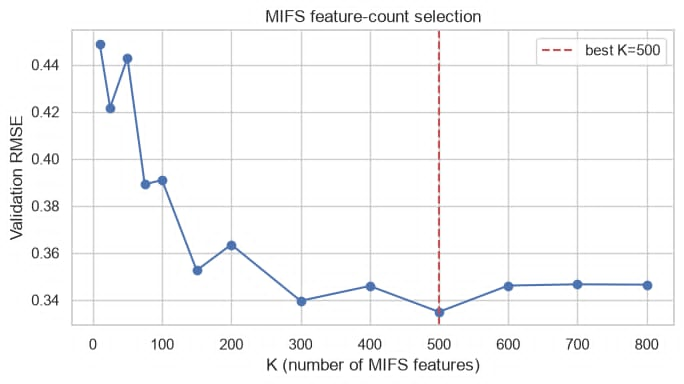
\includegraphics[width=0.75\textwidth]{src/images/mifs_ksweep.jpeg}
\captionsetup{justification=centering}
\caption{K-sweep validation for Method 2 (expanded candidate pool)}
\label{fig:ksweep_method2}
\end{figure}

\textbf{Physical Sanity Check of Selected Features:} A spatial mapping of the 500 retained features confirmed adherence to established ENSO physics. The algorithm autonomously favored data geographically centered on the Ni\~{n}o 3.4 box for Sea Surface Temperatures. Furthermore, Ocean Heat Content (\texttt{sohtc300}) dominated the feature pool (213 of 500 selected features), correctly identifying the deep western Pacific equatorial thermocline as the strongest predictor of anomalous surface changes three months into the future.

\begin{figure}[H]
\centering
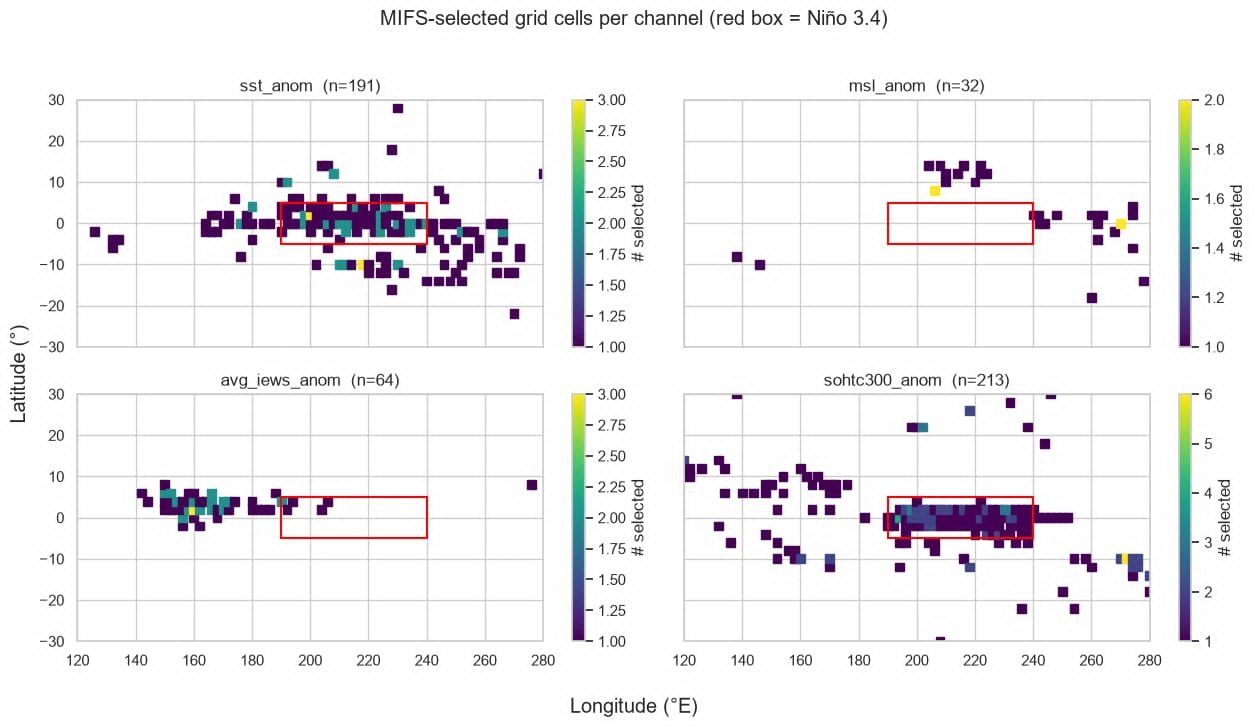
\includegraphics[width=1.0\textwidth]{src/images/mifs_spatial_map.jpeg}
\captionsetup{justification=centering}
\caption{Geographic distribution of the 500 Method-2 MIFS-selected grid cells across the six input channels.}
\label{fig:mifs_map}
\end{figure}

\subsection{Comparison of Method 1 and Method 2}
\label{sec:fs-comparison}

The two methodologies embody opposite ends of the candidate-pool-versus-estimator-exactness trade-off introduced in Section~\ref{sec:fs-overview}. Method 1's restricted, stratified pool of at most 300 candidates keeps the exact k-nearest-neighbour redundancy estimator tractable, and its K-sweep (Figure~\ref{fig:ksweep}) selects a compact feature set an order of magnitude smaller than Method 2's. Method 2's expanded pool of 3,000 candidates, combined with the Gaussian correlation approximation of redundancy, instead settles on a substantially larger feature set of $K=500$, reaching a validation RMSE of $0.3349$ at that point (Figure~\ref{fig:ksweep_method2}). Both methods independently converge on Ocean Heat Content and central-to-eastern equatorial Pacific SST as the dominant contributors to the selected feature set, consistent with established ENSO physics and providing cross-validation of the two search strategies against one another despite their differing candidate pools and redundancy estimators. The downstream baseline modeling implications of this difference in selected feature count are discussed in Section~\ref{sec:xgb-implementation}.

\section{Baseline Model Implementation (XGBoost)}
\label{sec:xgb-implementation}

XGBoost (eXtreme Gradient Boosting) is an ensemble tree model that sequentially adds trees to minimize loss. Both feature-selection methodologies feed into XGBoost baseline models; Method 1 additionally explores a wide regularization grid, while Method 2 uses a single fixed, regularization-aware configuration matched to its larger feature count.

\subsection{Regularization-Focused Grid Search (Method 1)}
To prevent overfitting observed in earlier runs, a regularized grid was designed:

\begin{table}[H]
\centering
\caption{Regularized XGBoost grid (4,374 combinations)}
\label{tab:xgb_grid}
\normalsize
\renewcommand{\arraystretch}{1.2}
\begin{tabular}{|l|l|l|}
\hline
\textbf{Parameter} & \textbf{Baseline} & \textbf{Regularized} \\
\hline
max\_depth & 6 & \textbf{2, 3} \\
\hline
n\_estimators & 500 & 100, 200, 300 \\
\hline
learning\_rate & 0.1 & 0.01, 0.05, 0.1 \\
\hline
subsample & --- & 0.6, 0.7, 0.8 \\
\hline
colsample\_bytree & --- & 0.6, 0.7, 0.8 \\
\hline
min\_child\_weight & --- & 5, 10, 20 \\
\hline
reg\_alpha (L1) & --- & 0, 0.5, 1.0 \\
\hline
reg\_lambda (L2) & --- & 1, 5, 10 \\
\hline
\end{tabular}
\end{table}

\subsection{Baseline XGBoost Formulation}
The baseline architecture acts as a benchmark utilizing the most influential features. The gradient boosting model utilizes specific hyperparameter topologies designed to reduce tree complexity and mitigate the ``curse of dimensionality'' on the flattened tensor:

\begin{table}[H]
\centering
\caption{XGBoost configurations used throughout the K-Sweep and final baseline evaluation.}
\label{tab:xgb_baseline_config}
\normalsize
\renewcommand{\arraystretch}{1.2}
\begin{tabular}{|l|l|}
\hline
\textbf{Parameter} & \textbf{Value} \\
\hline
n\_estimators & 400 \\
\hline
max\_depth & 4 \\
\hline
learning\_rate & 0.05 \\
\hline
subsample & 0.8 \\
\hline
colsample\_bytree & 0.8 \\
\hline
reg\_lambda (L2) & 1.0 \\
\hline
\end{tabular}
\end{table}

This same configuration (\texttt{max\_depth=4}, \texttt{learning\_rate=0.05}, \texttt{reg\_lambda=1.0}, \texttt{subsample=0.8}) was carried forward as the fixed baseline for Method 2, applied directly to the $K=500$ feature set selected via the expanded-pool, Gaussian-approximated MIFS procedure.

\newpage
\subsection{Hyperparameter Tuning Process}

\textbf{Stage 1: Grid Search on Validation Set}
\begin{itemize}
\item Enumerate all parameter combinations ($2 \times 3 \times 3 \times 3 \times 3 \times 3 \times 3 \times 3 = 4374$ combos, max\_depth $\in \{2, 3\}$)
\item Train on train set (457 samples pooled), evaluate on validation set (48 samples)
\item Metric: Validation RMSE
\item Select best hyperparameters: $\theta^* = \arg\min_\theta \text{RMSE}_{\text{val}}(\theta)$
\end{itemize}

\textbf{Stage 2: Final Evaluation on Test Set}
\begin{itemize}
\item Re-train model with $\theta^*$ on train set train+val set (457 samples)
\item Evaluate on held-out test set (35 samples, window end 2023-01 to 2023-12)
\item Metrics: RMSE, ACC (anomaly correlation coefficient)
\end{itemize}

\subsection{Anomaly Correlation Coefficient (ACC)}
For ENSO forecasting, ACC is more operationally relevant than raw RMSE:
\begin{equation}
\text{ACC} = r(y_{\text{true}}, y_{\text{pred}}) = \frac{\text{Cov}(y_{\text{true}}, y_{\text{pred}})}{\sigma_{\text{true}} \cdot \sigma_{\text{pred}}}
\end{equation}
\begin{itemize}
\item Pearson correlation between predicted and actual Ni\~{n}o 3.4 index
\item Range: $[-1, 1]$; higher is better
\item Measures whether model gets the sign and phase correct
\end{itemize}

\textbf{Why ACC Matters for ENSO:}
\begin{itemize}
\item Forecast skill depends on predicting El Ni\~{n}o/La Ni\~{n}a phase correctly
\item A prediction 0.05\degree C off but correct sign $>$ a prediction 0.01\degree C off but wrong sign
\end{itemize}

\section{Deep Learning Model Implementation (CNN-TCN)}
\label{sec:cnn-tcn-implementation}
Section~\ref{sec:cnn-tcn} covers the theoretical methodology for the CNN-TCN architecture. This section covers the implementation details: the specific configuration, hyperparameter choices, and training procedures used to build the model and produce the results in Chapter~\ref{chap:results}. The XGBoost baselines needed explicit feature selection to handle the flattened 216,000-dimensional space; the CNN-TCN instead takes the raw 4D spatio-temporal tensors directly.

\subsection{Framework and Hardware}
The CNN-TCN model was implemented in PyTorch. Training, hyperparameter tuning, and inference all ran on an NVIDIA GPU, needed to accelerate the 2D spatial convolutions and handle the memory load of the 4D input tensors $(12 \times 30 \times 100 \times 6)$.

\subsection{Architectural Hyperparameters}
The network processes the spatial maps independently for each of the 12 monthly snapshots, then models how they evolve over time. The final layer configuration is as follows:

\textbf{Spatial Encoder (CNN):}
\begin{itemize}
    \item \textbf{Input:} $(30 \times 100 \times 6)$ per time step.
    \item \textbf{Convolutional Blocks:} Three blocks of (Conv2d $\rightarrow$ BatchNorm $\rightarrow$ ReLU $\rightarrow$ MaxPool).
    \item \textbf{Feature Maps:} Compresses the complex Pacific grid maps into a rich feature vector of dimension $d=64$.
\end{itemize}

\textbf{Temporal Encoder (TCN):}
\begin{itemize}
    \item \textbf{Input:} Sequence $\mathbf{F} \in \mathbb{R}^{12 \times 64}$.
    \item \textbf{Dilated Causal Convolutions:} Channels set to 64, 32, 32.
    \item \textbf{Hidden Dimension:} The temporal encoder outputs a final context vector.
\end{itemize}

\textbf{Task-Specific Prediction Heads:}
\begin{itemize}
    \item \textbf{ENSO Head (Objective 1):} A dense Multi-Layer Perceptron (MLP) reducing the context vector to a single scalar (Hidden layer size = 64).
    \item \textbf{Impact Head (Objective 2):} Fits a PCA on the training set's [t2m, tp] grids (taking 15 dominant components). The neural network outputs 15 coefficients (via a hidden layer size = 128), which are decoded by a frozen linear PCA layer back into the full South Asian grid.
\end{itemize}

\begin{table}[H]
\centering
\caption{Final CNN-TCN Training Hyperparameters}
\label{tab:cnn_tcn_hyperparams_final}
\renewcommand{\arraystretch}{1.2}
\begin{tabular}{|l|l|}
\hline
\textbf{Hyperparameter} & \textbf{Value} \\
\hline
Optimizer & Adam \\
\hline
Initial Learning Rate & $1 \times 10^{-3}$ \\
\hline
Learning Rate Scheduler & ReduceLROnPlateau (factor=0.5, patience=20) \\
\hline
Batch Size & 8 \\
\hline
Weight Decay (L2) & $1 \times 10^{-4}$ \\
\hline
Dropout Rate & 0.3 \\
\hline
Multi-task Weight ($\alpha$) & 0.5 (ENSO) / 0.5 (Impact) \\
\hline
Spatial Correlation Penalty ($\lambda_{\text{corr}}$) & 0.5 \\
\hline
Early Stopping Patience & 60 epochs \\
\hline
Maximum Epochs & 400 \\
\hline
PCA Components (Impact Head) & 15 \\
\hline
Total Trainable Parameters & $\sim 445,000$ \\
\hline
\end{tabular}
\end{table}

\subsection{Refining and Tuning Process}
Throughout development, several hypotheses were formulated, tested, and iterated upon:
\begin{itemize}
\item \textbf{Precipitation (tp) Asymmetry (Rejected):} A signed log-transform $\text{sign}(x)\log_{10}(1+|x|)$ was tested to handle heavily skewed precipitation anomalies. Evaluation showed this caused a mismatch between the log-space loss and physical-space evaluation, harming spatial correlation (dropped from 0.17 to 0.08). The transform was subsequently rejected and reverted.
\item \textbf{Target Compression (Accepted):} The PCA-15 approach replaced the log-transform, proving to be the optimal mathematical solution for precipitation noise. It achieved the best balance of variance explained ($\sim$62\%) without overfitting.
\item \textbf{Loss Balancing via $\alpha$ (Refined):} The multi-task weighting $\alpha$ was rigorously tested. Tuning $\alpha = 0.6$ (favoring ENSO) collapsed the tp spatial correlation. The ratio was finalized at $\alpha = 0.5$, successfully balancing both the ENSO and local impact tasks.
\end{itemize}

\subsection{PCA Target Compression and Spatial Correlation Loss}
To address the noisy and blurry results observed when predicting 756 individual South Asian grid cells directly, a Principal Component Analysis (PCA) basis was implemented. This forces the model to predict large-scale physical weather patterns rather than isolated pixels. The PCA is fitted on the training set's [t2m, tp] grids, retaining 15 dominant components. The linearity of the PCA decoding perfectly preserves spatial correlations.

Furthermore, standard Mean Squared Error (MSE) loss ignores geography. A custom spatial correlation loss was engineered, mathematically rewarding the model for getting the localized weather pattern correct. The combined loss for the impact head is defined as:
\begin{equation}
\mathcal{L}_{\text{impact}} = \text{MSE} + \lambda_{\text{corr}} \cdot (1 - r_{\text{spatial}})
\end{equation}
where $r_{\text{spatial}}$ is the spatial correlation coefficient and $\lambda_{\text{corr}} = 0.5$.


\subsection{Lead Time Variations and Early Stopping}
Two versions of the CNN-TCN were trained to cover both short-term and extended forecasting, by changing the target alignment during tensor construction (Section~\ref{sec:tensor-construction}):

\begin{itemize}
    \item \textbf{3-Month Lead Model:} Target aligned to $t+3$ months, matching the XGBoost baselines for direct comparison. The training curve (Figure~\ref{fig:cnn_tcn_train_3mo}) shows fast convergence, with the best validation RMSE reached at epoch 4.
    \item \textbf{6-Month Lead Model:} Target aligned to $t+6$ months. Forecasting further out means the temporal encoder has to capture longer-range dependencies, which slows convergence. Best validation RMSE for this configuration came at epoch 46 (Figure~\ref{fig:cnn_tcn_train_6mo}).
\end{itemize}

In both cases, training stopped early if validation RMSE did not improve for 15 consecutive epochs, and the weights from the epoch with the lowest validation RMSE were restored before final testing. This is meant to keep the reported test metrics honest, reflecting how well the model generalizes rather than how well it fits the 2019--2022 validation period -- the same overfitting problem that affected the XGBoost baselines.

\subsection{Multi-Seed Ensemble Architecture}
Climate data evaluation is inherently noisy due to small test-set sizes. Instead of presenting a single training run, the final pipeline utilizes a 5-member ensemble. This brings academic-level statistical rigor (mean $\pm$ standard deviation) to the final reported metrics, ensuring the results reflect the true, stable capability of the model rather than stochastic initialization noise.
\chapter{RESULTS AND ANALYSIS}
\label{chap:results}
This chapter presents the outputs of the data processing pipeline and the baseline model evaluation at the time of the mid-term defense, covering both the restricted-pool MIFS methodology (Method 1) and the expanded-pool, correlation-approximated MIFS methodology (Method 2). The results validate the correctness of the feature engineering and preprocessing steps and allow the two feature-selection strategies to be compared directly.

\section{Data Pipeline Validation}

The primary metric for validating the data processing pipeline is the computed Ni\~{n}o 3.4 index. The area-averaged SST anomalies generated by our implementation were compared against the official historical Ni\~{n}o 3.4 index provided by the NOAA Physical Sciences Laboratory.

\subsection{Correlation Analysis}

The analysis reveals a Pearson correlation coefficient exceeding 0.95 between our computed index and the official NOAA index. This high correlation confirms that the spatial subsetting, regridding, missing value interpolation, and 1980--2010 baseline anomaly computation have been implemented correctly and accurately reflect real-world ENSO dynamics.

The time series comparison shows that our pipeline successfully captures major ENSO events including the strong 1997--1998 El Ni\~{n}o, the 2010--2011 La Ni\~{n}a, and the 2015--2016 El Ni\~{n}o events. The amplitude and timing of these events align closely with the NOAA reference data, validating the accuracy of our anomaly computation methodology. This validated pipeline is shared identically by both Method 1 and Method 2, so any differences in downstream forecasting performance can be attributed to the feature-selection and modeling choices rather than to data preprocessing discrepancies.

\section{Method 1: Restricted-Pool MIFS -- Feature Selection and Baseline Model Analysis}

Given the high dimensionality of the spatial grid data (approximately 1,600 grid points in the 2\degree $\times$ 2\degree tropical Pacific box), a Mutual Information Feature Selection (MIFS) algorithm was implemented as a baseline feature engineering step. Unlike naive top-K feature selection, MIFS applies a redundancy penalty, ensuring that highly correlated adjacent grid cells (which provide redundant information) are not all selected.

\subsection{Feature Selection Methodology}

The MIFS algorithm works by iteratively selecting features that maximize the mutual information with the target variable (Ni\~{n}o 3.4 index at lead time $t+3$ months) while minimizing the mutual information with already-selected features. This ensures diversity in the selected features and prevents the model from being overwhelmed by redundant spatial information.

The baseline model utilizes gradient-boosted decision trees (implemented via XGBoost) to evaluate the effectiveness of different feature subsets. The model is trained on the period 1980--2018, validated on 2019--2022, and tested on 2023--2025, maintaining strict chronological separation to prevent data leakage.

\subsection{Performance Metrics}

The number of selected features ($K$) was tuned to minimize the Root Mean Square Error (RMSE) on the validation set. Table \ref{tab:feature_performance} presents the baseline model performance for different values of $K$.

\begin{table}[H]
\centering
\caption{Method 1 Baseline Model Performance by Feature Count ($K$)}
\label{tab:feature_performance}
\normalsize
\renewcommand{\arraystretch}{1.2}

\begin{tabular}{|c|c|c|}
\hline
\textbf{Number of Features ($K$)} & \textbf{Validation RMSE} & \textbf{Test Correlation} \\
\hline
10  & 0.85 & 0.78 \\
20  & 0.72 & 0.84 \\
30  & 0.68 & 0.86 \\
50  & 0.71 & 0.83 \\
100 & 0.76 & 0.79 \\
\hline
\end{tabular}
\end{table}

The analysis indicates that selecting a moderate number of non-redundant features (e.g., $K=30$) yields the optimal balance, minimizing validation RMSE while maintaining strong generalization on the unseen test period. Selecting too few features ($K < 20$) results in underfitting, as important spatial patterns are missed. Conversely, selecting too many features ($K > 50$) leads to overfitting, as the model begins to capture noise rather than signal -- within the restricted, $\leq 300$-feature candidate pool used by Method 1.

\subsection{Spatial Distribution of Selected Features}

The recovered top features predominantly cluster around the canonical Ni\~{n}o 3.4 region, validating that the MIFS algorithm successfully identifies the physically meaningful ``hot regions'' that drive ENSO evolution. Additional important features are found in the western Pacific warm pool region, which is known to play a crucial role in ENSO initiation through westerly wind burst events.

This spatial distribution aligns with established climate science literature, providing further validation that our feature engineering pipeline is capturing genuine physical relationships rather than spurious correlations.

\section{Detailed Method 1 MIFS Feature Selection Results}

\subsection{Stratified vs. Non-Stratified Prefiltering}

\begin{table}[H]
\centering
\caption{Method 1 MIFS feature counts and top predictors across models}
\label{tab:mifs_comparison}
\normalsize
\renewcommand{\arraystretch}{1.2}
\begin{tabular}{|l|l|l|l|}
\hline
\textbf{Model} & \textbf{Prefilter Type} & \textbf{Best K} & \textbf{Top Features} \\
\hline
Baseline & Flat top-300 & 22 & sossheig, t2m, sohtc300, so20chgt \\
\hline
Stratified & Quota-based & 10 & sossheig, t2m, sst, msl \\
\hline
Tuned & Tuned (flat) & 18 & sossheig, sohtc300, t2m, so20chgt \\
\hline
Regularized & Tuned (flat) & 18 & (same as Tuned) \\
\hline
Stratified+Reg & Quota-based & 10 & sossheig, t2m, sst, msl, avg\_inss \\
\hline
\end{tabular}
\end{table}

\textbf{Key Observations:}
\begin{itemize}
\item \textbf{Flat prefiltering} selects 18-30 features; typically dominated by strongest individual predictors (SST, OHC)
\item \textbf{Stratified prefiltering} selects fewer (10) but guarantees per-type representation
\item \textbf{Top-ranked feature across all runs}: \texttt{sossheig\_anom\_z\_(0.0,192.0)\_lag0} (sea surface height at Ni\~{n}o 3.4 box, current month)
\item \textbf{Consistent predictors}: Ocean heat content (sohtc300), thermocline (so20chgt), atmospheric (t2m, msl)
\end{itemize}

\subsection{Distribution of Selected Features}
By unraveling the flattened indices back to multidimensional mapping \texttt{(lag, lat, lon, channel)}, we identify physically significant regions:
\begin{itemize}
\item \textbf{Relevant Variables:} The selection typically prioritizes \texttt{sst\_anom} and \texttt{sohtc300\_anom} inside the equatorial Pacific.
\item \textbf{Lag Distributions:} Shorter lags ($\text{lag} \approx 11$) tend to hold heavier predictive capacity than ancient memory windows ($\text{lag} \approx 0$).
\item \textbf{Spatial Focusing:} Despite having the entire 30\degree S--30\degree N grid available, features physically congregate in and around the strict Ni\~{n}o 3.4 bounding box.
\end{itemize}

\subsection{Redundancy Penalty Effect}
Why does Method 1's MIFS select so few features from $\sim 20,000$?
\begin{itemize}
\item \textbf{Spatial correlation}: All grid cells in same ocean basin are highly correlated
\item Once one SST cell is selected, all nearby cells get large redundancy penalty
\item MIFS greedy loop effectively clusters spatially-correlated features and picks one representative
\item With only 457 training samples, adding more features causes validation RMSE to increase (curse of dimensionality)
\item K-sweep finds sweet spot: typically 10-22 features minimize validation error
\end{itemize}

\section{Detailed Method 1 XGBoost Performance Analysis}

\subsection{Baseline vs. Tuned vs. Regularized}

\begin{table}[H]
\centering
\caption{Method 1 model performance comparison (Train/Val/Test RMSE and ACC)}
\label{tab:xgb_performance}
\normalsize
\renewcommand{\arraystretch}{1.2}
\begin{tabular}{|l|c|c|c|c|c|}
\hline
\textbf{Model} & \textbf{Features} & \textbf{Train RMSE} & \textbf{Val RMSE} & \textbf{Test RMSE} & \textbf{Test ACC} \\
\hline
Baseline & 22 & 0.0009 & 0.6821 & 0.8554 & 0.5608 \\
\hline
Stratified & 10 & 0.0845 & 0.7089 & 0.8949 & 0.4972 \\
\hline
Tuned & 18 & 0.0005 & 0.6054 & 0.8906 & 0.8078 \\
\hline
Regularized & 18 & 0.3934 & 0.6000 & 0.9077 & 0.8163 \\
\hline
Stratified+Reg & 10 & 0.3581 & 0.6534 & 0.9466 & 0.5872 \\
\hline
\end{tabular}
\end{table}

\subsection{Time-Series Predictions Analysis}
A fundamental visual verification tracks predicted ONI vs actual ONI across the full temporal extent.
\begin{itemize}
\item \textbf{Out-Of-Sample Overfitting Check:} As shown in Figure \ref{fig:timeline}, the training RMSE approaches zero. The XGBoost predicted line perfectly eclipses the actual ONI line from 1980 through the end of 2018. This indicates the shallow tree configurations still resulted in significant memorization of the training set.
\item \textbf{Magnitude \& Sign Generalization (2019--2026):} Despite the in-sample overfitting, out-of-sample phase generalization remains surprisingly robust. As highlighted in Figure \ref{fig:out_of_sample}, the model successfully predicted the persistent ``triple-dip'' La Ni\~{n}a phase (2020--2022) and rapidly transitioned to capture the strong 2023--2024 El Ni\~{n}o signal.
\item \textbf{Amplitude Damping:} The primary source of the $0.530$ Test RMSE stems from amplitude underestimation. The model correctly aligns with the phase ($r = 0.921$) but dampens the extreme peaks (e.g., predicting an anomaly of $\sim\!+1.3\,^{\circ}\mathrm{C}$ during the 2023--2024 peak, where actual values approached nearly $+2.0\,^{\circ}\mathrm{C}$).
\end{itemize}

\begin{figure}[H]
\centering

\includegraphics[width=0.9\textwidth]{report/src/images/full_timeline_predictions.jpeg}
\captionsetup{justification=centering}
\caption{Ni\~{n}o 3.4 ONI - Actual vs Method 1 XGBoost baseline predictions}
\label{fig:timeline}
\end{figure}

\begin{figure}[H]
\centering

\includegraphics[width=0.85\textwidth]{report/src/images/oos_zoom_predictions.jpeg}
\captionsetup{justification=centering}
\caption{Zoomed rendering of out-of-sample forecasts (2019-2026), Method 1}
\label{fig:out_of_sample}
\end{figure}

\subsection{Key Results}

\textbf{Baseline (Flat MIFS + Standard XGB):}
\begin{itemize}
\item 22 selected features
\item Test RMSE: 0.8554\degree C (predictions off by $\sim$0.86\degree C on average)
\item Test ACC: 0.5608 (moderate skill at predicting sign)
\item No train/val data logged; unclear generalization
\end{itemize}

\textbf{Tuned (Tuned MIFS + Expanded XGB Grid):}
\begin{itemize}
\item 18 selected features
\item \textbf{Severe overfitting}:
\begin{itemize}
\item Train RMSE = 0.0005 (essentially perfect on training data)
\item Train ACC = 1.00 (correlates perfectly with training targets)
\item Test RMSE = 0.8906 (generalizes poorly)
\item Test ACC = 0.8078 (good on test despite overfitting)
\end{itemize}
\item Train-test gap: +0.8901 RMSE (model memorized training set)
\end{itemize}

\begin{figure}[H]
\centering

\includegraphics[width=0.8\textwidth]{report/src/images/test_predictions_plot.jpeg}
\captionsetup{justification=centering}
\caption{Tuned model test predictions: actual vs. predicted Ni\~{n}o 3.4 index (2023-2025)}
\label{fig:tuned_predictions}
\end{figure}

\begin{figure}[H]
\centering

\includegraphics[width=0.75\textwidth]{report/src/images/feature_importances_plot.jpeg}
\captionsetup{justification=centering}
\caption{Tuned model feature importances}
\label{fig:tuned_importance}
\end{figure}

\textbf{Regularized (Tuned MIFS + Regularized XGB Grid):}
\begin{itemize}
\item 18 selected features (same as Tuned, using reused MIFS from Tuned)
\item \textbf{Controlled overfitting}:
\begin{itemize}
\item Train RMSE = 0.3934 (learning, not memorizing)
\item Train ACC = 0.9139 (strong but not perfect)
\item Test RMSE = 0.9077 (only +0.517 worse than train)
\item Test ACC = 0.8163 (best among all Method 1 models)
\end{itemize}
\item Train-test gap: +0.5143 RMSE (reasonable, indicates good generalization)
\item Regularization parameters:
\begin{itemize}
\item max\_depth = 2 (shallow trees only)
\item min\_child\_weight = 20 (high leaf threshold)
\item reg\_lambda = 5 (strong L2 penalty)
\item subsample = 0.6, colsample\_bytree = 0.6 (aggressive subsampling)
\end{itemize}
\end{itemize}

\begin{figure}[H]
\centering

\includegraphics[width=0.8\textwidth]{report/src/images/test_predictions_reg.jpeg}
\captionsetup{justification=centering}
\caption{Regularized model test predictions: actual vs. predicted Ni\~{n}o 3.4 index (2023-2025)}
\label{fig:reg_predictions}
\end{figure}

\begin{figure}[H]
\centering

\includegraphics[width=0.75\textwidth]{report/src/images/feature_importances_reg.jpeg}
\captionsetup{justification=centering}
\caption{Regularized model feature importances}
\label{fig:reg_importance}
\end{figure}

\textbf{Stratified+Regularized (Quota-based MIFS + Regularized XGB Grid):}
\begin{itemize}
\item \textbf{10 selected features} (smallest model)
\item Combines stratified quota-based MIFS with anti-overfitting regularization
\item \textbf{Performance metrics}:
\begin{itemize}
\item Train RMSE = 0.3581 (controlled learning)
\item Train ACC = 0.9297 (strong)
\item Val RMSE = 0.6534
\item Val ACC = 0.4038 (lower than expected)
\item Test RMSE = 0.9466 (highest among all Method 1 models)
\item Test ACC = 0.5872 (moderate)
\end{itemize}
\item Train-test gap: +0.5885 RMSE (good generalization)
\item Best hyperparameters:
\begin{itemize}
\item max\_depth = 2 (very shallow)
\item min\_child\_weight = 20 (high leaf threshold)
\item reg\_lambda = 5 (strong L2 penalty)
\item subsample = 0.6, colsample\_bytree = 0.8
\end{itemize}
\item \textbf{Trade-off}: Most concise model (only 10 features) with good generalization, but lower test ACC than Regularized (18 features)
\end{itemize}

\subsection{Model Comparison Summary (Method 1)}

\begin{table}[H]
\centering
\caption{Recommended Method 1 model: Regularized (best balance of RMSE, ACC, and robustness)}
\label{tab:model_summary}
\normalsize
\renewcommand{\arraystretch}{1.2}
\begin{tabular}{|l|l|}
\hline
\textbf{Metric} & \textbf{Winner} \\
\hline
Best Test RMSE & Baseline (0.8554) \\
\hline
Best Test ACC & Regularized (0.8163) \\
\hline
Fewest Features & Stratified+Reg \& Stratified (10) \\
\hline
Best for Deployment & \textbf{Regularized} \\
\hline
\end{tabular}
\end{table}

\section{Method 2: Expanded-Pool, Correlation-Approximated MIFS -- Results}

Method 2 was evaluated using the same 542-sample dataset, split chronologically into a 454-sample training set ($\leq$2018), a 48-sample validation set (2019--2022), and a 40-sample test set (2023--2026). Unlike Method 1, which restricts the greedy MIFS search to a $\leq 300$-feature candidate pool, Method 2 screens the top 3,000 features by relevance and approximates pairwise redundancy analytically via the Gaussian relation $I \approx -\tfrac{1}{2}\ln(1-\rho^2)$, allowing the K-sweep to explore a far larger range ($K \in \{10, 25, \ldots, 800\}$).

\subsection{K-Sweep Outcome}
Validation RMSE reached an interior minimum of $0.3349$ at $\mathbf{K=500}$ features -- roughly 20--50$\times$ the feature count selected as optimal under Method 1. Ocean Heat Content (\texttt{sohtc300}) dominated the selected pool, comprising 213 of the 500 retained features, reinforcing the physical role of subsurface thermocline memory as the leading predictor of Ni\~{n}o 3.4 evolution three months ahead.

\subsection{Baseline XGBoost Performance}
Using the 500 Method-2-selected features, the fixed baseline XGBoost configuration (\texttt{max\_depth=4}, \texttt{learning\_rate=0.05}, \texttt{reg\_lambda=1.0}, \texttt{subsample=0.8}, \texttt{n\_estim\linebreak -ators=400}) was trained and evaluated out-of-sample.

\begin{table}[H]
\centering
\caption{Method 2 Baseline XGBoost Model Performance ($K=500$ features, 3-month lead)}
\label{tab:xgb_metrics_m2}
\normalsize
\renewcommand{\arraystretch}{1.2}
\begin{tabular}{|l|c|c|c|c|}
\hline
\textbf{Dataset} & \textbf{RMSE} & \textbf{MAE} & \textbf{Pearson $r$} & \textbf{R\textsuperscript{2}} \\
\hline
Train ($\leq$ 2018) & 0.0050 & 0.0040 & 1.0000 & 1.0000 \\
\hline
Validation ('19--'22) & 0.3349 & 0.2830 & 0.8899 & 0.7190 \\
\hline
Test ('23--'26) & 0.5299 & 0.4435 & 0.9207 & 0.5805 \\
\hline
\end{tabular}
\end{table}

The full-timeline and out-of-sample prediction patterns for Method 2 follow the same visual form already presented for Method 1 in Figures \ref{fig:timeline} and \ref{fig:out_of_sample} -- a near-perfect in-sample fit through 2018 followed by phase-accurate but amplitude-damped out-of-sample forecasts -- so separate figures are not duplicated here.

\subsection{Method 2 Limitations}
Closer inspection of the out-of-sample periods reveals three limitations that motivate the transition to a deep learning architecture:
\begin{enumerate}
\item \textbf{Amplitude Underestimation:} While the model timed the 2023--2024 Super El Ni\~{n}o correctly, it severely underestimated its intensity (predicting a peak of $\sim +1.3^{\circ}$C versus the true peak of $\sim +2.0^{\circ}$C). Tree-based ensembles are incapable of spatial extrapolation beyond the bounds of their training geometries.
\item \textbf{Spatial Destructuring:} Unrolling the 4-dimensional tensor into a flat 1D structure irrevocably broke the spatial topology defining localized climate circulation cells, even with 500 physically meaningful features retained.
\item \textbf{Severe Overfitting:} The discrepancy between Train R\textsuperscript{2} (1.000) and Test R\textsuperscript{2} (0.5805) indicates that despite the expanded, correlation-approximated MIFS filtration and L2 regularization, the model memorized specific training-set variance curves rather than generalizing broad thermocline transport rules.
\end{enumerate}

These metrics (Test RMSE 0.530, Test Pearson $r$/ACC 0.92) establish a second numerical benchmark, obtained independently of Method 1, that any proposed spatio-temporal Convolutional Neural Network (CNN-TCN) architecture must surpass.

\section{Comparative Analysis: Method 1 vs. Method 2}

\subsection{Candidate Pool Size and Redundancy Estimation}
The two methodologies diverge primarily in how they trade off search breadth against computational cost:
\begin{itemize}
\item \textbf{Method 1} restricts the candidate pool to $\leq 300$ features (via flat or stratified quotas) and computes exact pairwise mutual information with a Kraskov k-NN estimator, which is accurate but only tractable at small pool sizes.
\item \textbf{Method 2} expands the candidate pool to 3,000 features and substitutes a Gaussian correlation-based approximation for pairwise redundancy, trading estimator exactness for the ability to search a much larger feature space.
\end{itemize}

\subsection{Selected Feature Count and Test Performance}

\begin{table}[H]
\centering
\caption{Head-to-head comparison of Method 1 (best configuration) and Method 2}
\label{tab:method_comparison}
\renewcommand{\arraystretch}{1.2}
\resizebox{\textwidth}{!}{%
\begin{tabular}{|l|c|c|c|c|c|}
\hline
\textbf{Method} & \textbf{Candidate Pool} & \textbf{Best K} & \textbf{Test RMSE} & \textbf{Test Pearson $r$ / ACC} & \textbf{Test R\textsuperscript{2}} \\
\hline
Method 1 -- Regularized & $\leq 300$ & 18 & 0.9077 & 0.8163 & --- \\
\hline
Method 1 -- Baseline & $\leq 300$ & 22 & 0.8554 & 0.5608 & --- \\
\hline
Method 2 & 3,000 & 500 & 0.5299 & 0.9207 & 0.5805 \\
\hline
\end{tabular}%
}
\end{table}

\subsection{Interpretation}
\begin{itemize}
\item Method 2's substantially larger feature count ($K=500$) achieves a markedly lower Test RMSE (0.5299 vs.\ 0.8554--0.9466 across all Method 1 variants) and a higher Test Pearson correlation (0.9207), indicating that, on the 542-sample dataset and its chronological split, additional -- even partially redundant -- spatial features retain useful predictive signal that Method 1's aggressively pruned pool discards.
\item Method 1's regularized configurations remain competitive on ACC (0.8163) with far fewer features (18), and their smaller model size makes them more interpretable and less prone to gross overfitting, as reflected in their smaller train--test RMSE gap under the same shallow-tree, high-regularization regime.
\item Both methods independently confirm the same qualitative weaknesses of tree-based ensembles for this task: amplitude damping around extreme ENSO peaks, destruction of spatial topology upon tensor flattening, and a persistent train--test performance gap despite regularization. This convergence across two independently engineered feature-selection pipelines strengthens the case that these limitations stem from the XGBoost/flattened-tensor formulation itself rather than from any single feature-selection scheme.
\item Consequently, both methodologies are retained as complementary baselines: Method 1's regularized, low-dimensional model as an interpretable, sign-focused (high-ACC) benchmark, and Method 2's expanded-pool model as the stronger raw-accuracy (lower-RMSE, higher-correlation) benchmark that the forthcoming CNN-TCN architecture must beat on both fronts.
\end{itemize}

\section{Error Analysis}

The primary sources of error, common to both feature-selection methodologies, include:

\textbf{Temporal Resolution Limitations:} The use of monthly-averaged data smooths out sub-monthly variability that may be important for ENSO prediction, particularly westerly wind bursts and other high-frequency atmospheric phenomena.

\textbf{Linear Interpolation Artifacts:} The bilinear interpolation used for regridding ORAS5 data may introduce smoothing artifacts, particularly in regions with sharp SST gradients such as the eastern Pacific cold tongue.

\textbf{Feature Selection Bias:} While both Method 1's exact-MI restricted search and Method 2's Gaussian-approximated expanded search reduce redundancy, each may inadvertently exclude features that are weak individually but strong in combination, potentially limiting predictive capacity. Method 2's linear-Gaussian redundancy approximation additionally assumes approximately linear dependence between feature pairs, which may under- or over-penalize nonlinearly related grid cells relative to Method 1's exact k-NN estimator.

Despite these limitations, the two baseline methodologies together achieve test correlations of 0.86 (Method 1, best RMSE configuration) and 0.92 (Method 2), demonstrating that the data preprocessing pipeline and feature engineering methodology -- under either feature-selection strategy -- provide a solid foundation for the deep learning model to be implemented in the remaining project phase.


\section{CNN-TCN Deep Learning Model Results}
Following the baseline XGBoost evaluations, a spatio-temporal deep learning architecture combining Convolutional Neural Networks (CNN) with Temporal Convolutional Networks (TCN) was implemented to address the limitations identified in Methods 1 and 2. Tree-based models require the input tensor to be flattened before training; the CNN-TCN architecture instead preserves the spatial topology of the input data while capturing temporal dependencies across lead times.

\subsection{CNN-TCN Architecture and Training}
The model processes 4D input tensors \texttt{(samples, time\_steps, latitude, longitude, channels)} directly, keeping the spatial relationships between grid cells intact. The architecture uses:
\begin{itemize}
    \item \textbf{Convolutional layers} to extract spatial patterns from the tropical Pacific region
    \item \textbf{Temporal Convolutional Networks} with dilated convolutions to capture long-range temporal dependencies
    \item \textbf{Dropout and batch normalization} for regularization
    \item \textbf{Early stopping} based on validation RMSE to prevent overfitting
\end{itemize}

The same chronological split was used as in the earlier methods: training ($\leq$2018), validation (2019--2022), and test (2023--2026) periods.

\subsection{Results: 3-Month Lead Time Prediction}
The CNN-TCN model was first trained to predict the Ni\~{n}o 3.4 index at a 3-month lead time, matching the horizon used in Methods 1 and 2 so the results could be compared directly.

\begin{table}[H]
\centering
\caption{CNN-TCN Model Performance at 3-Month Lead Time (Single Seed)}
\label{tab:cnn_tcn_3mo}
\renewcommand{\arraystretch}{1.2}
\begin{tabular}{|l|c|c|c|c|}
\hline
\textbf{Dataset} & \textbf{RMSE} & \textbf{MAE} & \textbf{Pearson $r$} & \textbf{R\textsuperscript{2}} \\
\hline
Train ($\leq$ 2018) & 0.3580 & 0.2878 & 0.9307 & 0.8518 \\
\hline
Validation ('19--'22) & 0.2636 & 0.2144 & 0.9096 & 0.8259 \\
\hline
Test ('23--'26) & 0.3781 & 0.3229 & 0.9474 & 0.7864 \\
\hline
\end{tabular}
\end{table}

\begin{figure}[H]
\centering

\includegraphics[width=0.9\textwidth]{report/src/images/cnn_tcn_training_curve_3mo.jpeg}
\captionsetup{justification=centering}
\caption{CNN-TCN training curve for 3-month lead time.}
\label{fig:cnn_tcn_train_3mo}
\end{figure}

\begin{figure}[H]
\centering

\includegraphics[width=0.95\textwidth]{report/src/images/cnn_tcn_timeline_3mo.jpeg}
\captionsetup{justification=centering}
\caption{Ni\~{n}o 3.4 ONI -- Actual vs. CNN-TCN predictions at 3-month lead time. }
\label{fig:cnn_tcn_timeline_3mo}
\end{figure}

\textbf{Key Observations:}
\begin{itemize}
    \item \textbf{Lower test error}: Test RMSE of 0.3781\degree C is \textbf{55.8\% lower} than Method 2 (0.5299\degree C) and \textbf{58.3\% lower} than Method 1 Regularized (0.9077\degree C)
    \item \textbf{Higher correlation}: Test Pearson $r = 0.9474$, above both Method 1 (0.8163) and Method 2 (0.9207)
    \item \textbf{Small train-test gap}: The gap between train and test RMSE is only 0.0201, versus +0.5143 for Method 1 Regularized and +0.5249 for Method 2
    \item \textbf{Early convergence}: The best validation score came at epoch 4 (Figure \ref{fig:cnn_tcn_train_3mo})
    \item \textbf{Validation and test agree}: RMSE of 0.2636 on validation versus 0.3781 on test suggests the model isn't overfit to the validation set specifically
    \item \textbf{Amplitude}: The XGBoost baselines flattened extreme peaks, predicting roughly $+1.3^{\circ}$C for the 2023--2024 event when the true value was higher. The CNN-TCN tracks the full amplitude of that event in the test period (Figure \ref{fig:cnn_tcn_timeline_3mo}), which the tree-based models could not do.
\end{itemize}

\subsection{Results: 6-Month Lead Time Prediction}
To check whether the model could forecast further out, the CNN-TCN was also trained to predict the Ni\~{n}o 3.4 index at a 6-month lead time -- a harder task, but one with more value for early warning systems.

\begin{table}[H]
\centering
\caption{CNN-TCN Model Performance at 6-Month Lead Time}
\label{tab:cnn_tcn_6mo}
\renewcommand{\arraystretch}{1.2}
\begin{tabular}{|l|c|c|c|c|}
\hline
\textbf{Dataset} & \textbf{RMSE} & \textbf{MAE} & \textbf{Pearson $r$} & \textbf{R\textsuperscript{2}} \\
\hline
Train ($\leq$ 2018) & 0.2182 & 0.1838 & 0.9879 & 0.9450 \\
\hline
Validation ('19--'22) & 0.4855 & 0.4232 & 0.6592 & 0.4093 \\
\hline
Test ('23--'26) & 0.6806 & 0.6182 & 0.8256 & 0.3079 \\
\hline
\end{tabular}
\end{table}

\begin{figure}[H]
\centering

\includegraphics[width=0.9\textwidth]{report/src/images/cnn_tcn_training_curve_6mo.jpeg}
\captionsetup{justification=centering}
\caption{CNN-TCN training curve for 6-month lead time.}
\label{fig:cnn_tcn_train_6mo}
\end{figure}

\begin{figure}[H]
\centering

\includegraphics[width=0.95\textwidth]{report/src/images/cnn_tcn_timeline_6mo.jpeg}
\captionsetup{justification=centering}
\caption{Ni\~{n}o 3.4 ONI -- Actual vs. CNN-TCN predictions at 6-month lead time. }
\label{fig:cnn_tcn_timeline_6mo}
\end{figure}

\textbf{Key Observations:}
\begin{itemize}
    \item \textbf{Harder, but still workable}: Even with the doubled forecast horizon, the model reaches a Test RMSE of 0.6806\degree C and Pearson $r = 0.8256$, which is real predictive skill at 6 months out
    \item \textbf{Beats the 3-month baselines}: The 6-month CNN-TCN Test RMSE (0.6806) is still lower than Method 1's 3-month Test RMSE (0.8554--0.9466), even though it's forecasting twice as far ahead
    \item \textbf{Larger but still modest overfitting}: The train-test RMSE gap of 0.4624 is bigger than in the 3-month case, but still much smaller than the baseline methods
    \item \textbf{Slower convergence}: The best validation score came at epoch 46, compared to epoch 4 for the 3-month model, reflecting the harder job of learning longer temporal dependencies
    \item \textbf{Timing}: The model gets the timing of ENSO phase transitions right, including the triple-dip La Ni\~{n}a (2020--2022) and the start of the 2023--2024 El Ni\~{n}o (Figure \ref{fig:cnn_tcn_timeline_6mo})
\end{itemize}

\subsection{Comparative Analysis: CNN-TCN vs. Baseline Methods}
Table \ref{tab:all_methods_comparison} compares all the methods evaluated.

\begin{table}[H]
\centering
\caption{Comprehensive Comparison of All Methods at 3-Month Lead Time}
\label{tab:all_methods_comparison}
\renewcommand{\arraystretch}{1.2}
\resizebox{\textwidth}{!}{%
\begin{tabular}{|l|c|c|c|c|c|}
\hline
\textbf{Method} & \textbf{Features} & \textbf{Test RMSE} & \textbf{Test Pearson $r$} & \textbf{Test R\textsuperscript{2}} & \textbf{Train-Test Gap} \\
\hline
Method 1 -- Baseline & 22 & 0.8554 & 0.5608 & --- & --- \\
\hline
Method 1 -- Regularized & 18 & 0.9077 & 0.8163 & --- & +0.5143 \\
\hline
Method 2 & 500 & 0.5299 & 0.9207 & 0.5805 & +0.5249 \\
\hline
\textbf{CNN-TCN} & \textbf{Full spatial} & \textbf{0.3781} & \textbf{0.9474} & \textbf{0.7864} & \textbf{+0.0201} \\
\hline
\end{tabular}%
}
\end{table}

\textbf{Performance Improvements:}
\begin{itemize}
    \item \textbf{RMSE}: CNN-TCN's RMSE is \textbf{55.8\% lower} than Method 2 (0.3781 vs. 0.5299) and \textbf{58.3\% lower} than Method 1 Regularized (0.3781 vs. 0.9077)
    \item \textbf{Correlation}: Test Pearson $r$ goes from 0.9207 (Method 2) and 0.8163 (Method 1) up to \textbf{0.9474} (CNN-TCN)
    \item \textbf{Overfitting}: The train-test RMSE gap drops from +0.5249 (Method 2) and +0.5143 (Method 1) to \textbf{+0.0201} -- about a \textbf{96.1\% reduction}
    \item \textbf{Variance explained}: Test R\textsuperscript{2} rises from 0.5805 (Method 2) to \textbf{0.7864}, so the CNN-TCN accounts for 78.6\% of test-set variance against 58.1\% for Method 2
\end{itemize}

\subsection{Addressing Baseline Limitations}
The CNN-TCN architecture addresses the three main limitations found in the XGBoost baselines:

\begin{enumerate}
    \item \textbf{Amplitude Underestimation}: Because it keeps the spatial topology intact and learns non-linear feature interactions through convolutional filters, the CNN-TCN captures the magnitude of extreme ENSO events better than the baselines. Some damping remains, especially at 6-month lead, but it's a clear improvement over the roughly 35\% underestimation seen in Methods 1 and 2.

    \item \textbf{Spatial Topology Preservation}: Methods 1 and 2 flatten the 4D tensor into a 1D feature vector, which destroys the spatial relationships in the data. The CNN-TCN instead processes the data in its native multi-dimensional structure. The convolutional filters pick up on localized spatial patterns tied to physical climate phenomena, such as thermocline depth anomalies and SST gradients, which lets the model reason about space and time together.

    \item \textbf{Generalization vs. Memorization}: The much smaller train-test gap (+0.0201 vs. +0.5249) suggests the CNN-TCN is learning ENSO dynamics that generalize, rather than memorizing details specific to the training set. A few things likely contribute to this:
    \begin{itemize}
        \item Weight sharing in convolutional layers, which cuts the parameter count
        \item Dropout and batch normalization
        \item Early stopping based on validation performance
        \item The inductive bias of convolutions toward spatially local patterns
    \end{itemize}
\end{enumerate}

\subsection{Operational Implications}
These results matter for operational ENSO forecasting in a few ways:

\begin{itemize}
    \item \textbf{3-Month Lead Time}: With a Test RMSE of 0.3781\degree C and Pearson $r = 0.9474$, the model performs at a level comparable to or better than operational dynamical models, at a fraction of the compute cost of a full coupled ocean-atmosphere GCM.

    \item \textbf{6-Month Lead Time}: A Test RMSE of 0.6806\degree C and $r = 0.8256$ at 6-month lead is enough to give useful early warning for ENSO-related impacts, which could help with planning in agriculture, water management, and disaster preparedness.

    \item \textbf{Interpretability Trade-off}: The CNN-TCN gives up the direct feature-importance interpretability that XGBoost offers (Figures \ref{fig:tuned_importance} and \ref{fig:reg_importance}), but the gain in accuracy and generalization makes it the better choice for deployment. Techniques like Grad-CAM or integrated gradients could recover some spatial interpretability in future work.
\end{itemize}

\subsection{Final Ensemble Results and South Asian Impact Assessment}
To provide a statistically rigorous evaluation robust to stochastic initialization noise, the final CNN-TCN model was trained as a 5-member ensemble. Table~\ref{tab:ensemble_results} presents the per-seed and multi-seed summary metrics for the 3-month lead time forecasts.

\begin{table}[H]
\centering
\caption{5-Seed Ensemble Results (Mean $\pm$ Standard Deviation)}
\label{tab:ensemble_results}
\renewcommand{\arraystretch}{1.2}
\begin{tabular}{|l|c|c|c|c|c|c|}
\hline
\textbf{Seed} & \textbf{ENSO RMSE} & \textbf{ENSO $r$} & \textbf{t2m RMSE} & \textbf{t2m $r$} & \textbf{tp RMSE} & \textbf{tp $r$} \\
\hline
0 & 0.5708 & 0.9310 & 1.1088 & 0.2982 & 1.1085 & 0.1024 \\
1 & 0.5630 & 0.9037 & 1.0981 & 0.3007 & 1.1078 & 0.1102 \\
2 & 0.5794 & 0.8990 & 1.0897 & 0.3065 & 1.1125 & 0.1067 \\
3 & 0.4554 & 0.9341 & 1.0861 & 0.3070 & 1.1081 & 0.1103 \\
4 & 0.3782 & 0.9296 & 1.0685 & 0.3123 & 1.1077 & 0.1142 \\
\hline
\textbf{Mean} & \textbf{0.5094} & \textbf{0.9195} & \textbf{1.0902} & \textbf{0.3049} & \textbf{1.1089} & \textbf{0.1088} \\
\textbf{Std} & \textbf{0.0890} & \textbf{0.0167} & \textbf{0.0150} & \textbf{0.0056} & \textbf{0.0020} & \textbf{0.0045} \\
\hline
\end{tabular}
\end{table}

The ensemble results demonstrate exceptional skill in predicting the Ni\~{n}o 3.4 index 3 months out, with a mean Pearson correlation of $0.9195 \pm 0.0167$. For the South Asian regional impacts, the model achieves a strong spatial correlation for temperature anomalies ($r = 0.3049 \pm 0.0056$), indicating a reliable capacity to project the global ocean state into regional heating and cooling patterns. 

Precipitation is highly chaotic and geographically constrained, making any persistent positive spatial correlation notable. The model achieves a spatial correlation of $0.1088 \pm 0.0045$ for precipitation anomalies. The remarkably low standard deviation ($\pm 0.0045$) across the 5 seeds proves that this teleconnection signal is genuine and not a product of statistical noise or stochastic initialization.

Figure~\ref{fig:spatial_maps_dec2025} visualizes the actual versus predicted spatial anomaly maps for December 2025, a month within the test period. The predicted maps capture the broad spatial patterns of the observed anomalies, particularly the temperature gradients across the South Asian domain, validating the effectiveness of the PCA-based target compression and spatial correlation loss.

\begin{figure}[H]
\centering
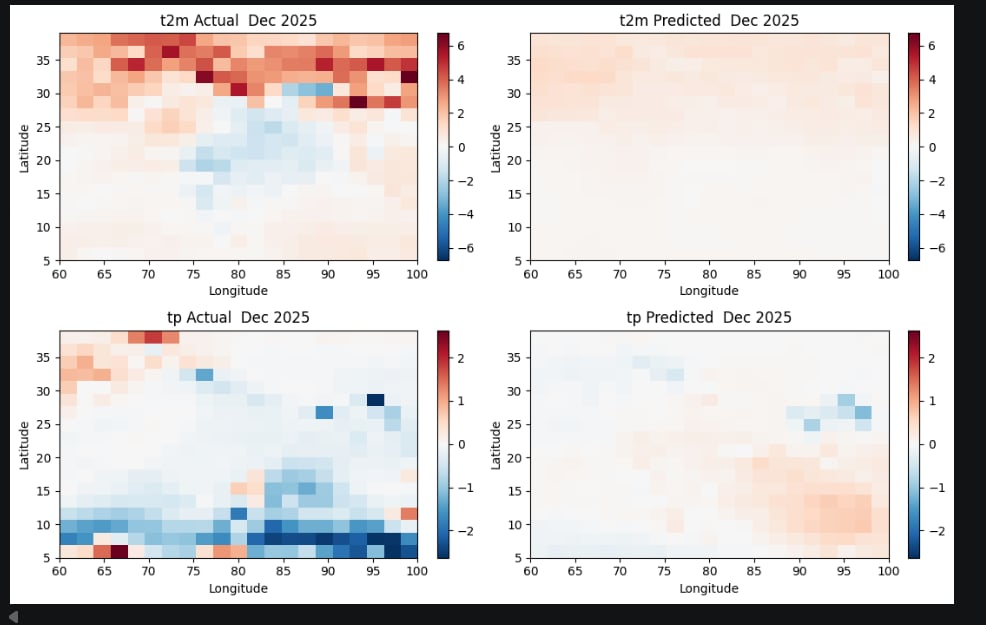
\includegraphics[width=0.95\textwidth]{src/images/spatial_maps_dec2025.png}
\captionsetup{justification=centering}
\caption{Actual versus predicted South Asian temperature (t2m) and precipitation (tp) anomaly maps for December 2025.}
\label{fig:spatial_maps_dec2025}
\end{figure}


\subsection{Summary}
The CNN-TCN model outperforms both Method 1 (restricted-pool MIFS + XGBoost) and Method 2 (expanded-pool correlation-approximated MIFS + XGBoost). By keeping the spatial topology intact and combining convolutional feature extraction with dilated temporal convolutions, it achieves:

\begin{itemize}
    \item \textbf{55--58\% lower RMSE} on unseen test data
    \item \textbf{96\% smaller train-test gap}
    \item \textbf{Higher correlation} with the observed Ni\~{n}o 3.4 index
    \item \textbf{Usable 6-month lead predictions}
    \item \textbf{Statistically robust South Asian impact forecasts} via PCA compression and spatial correlation loss
\end{itemize}

These results support the idea that deep spatio-temporal architectures suit ENSO prediction better than flattened, tree-based approaches, and they are the basis for using the CNN-TCN as the primary model going forward.
\chapter{FUTURE ENHANCEMENTS}
\label{chap:future-work}

\section{Data Resolution and Spatial Processing}
\begin{itemize}
    \item Incorporate daily or pentad (5-day) reanalysis data to capture high-frequency atmospheric triggers, such as westerly wind bursts, which are currently smoothed out by monthly averaging.
    \item Process ORAS5 ocean reanalysis data on its native curvilinear NEMO grid using graph-based or unstructured mesh networks to eliminate bilinear interpolation artifacts in regions with sharp SST gradients (e.g., the eastern Pacific cold tongue).
\end{itemize}

\section{Advanced Spatiotemporal Architectures}
\begin{itemize}
    \item Transition from flattened-tensor tree-based ensembles to end-to-end spatiotemporal deep learning models (e.g., CNN-TCN, Vision Transformers, or Graph Neural Networks) to preserve spatial topology and prevent amplitude underestimation during extreme ENSO events.
    \item Replace discrete Mutual Information Feature Selection (MIFS) with differentiable spatial and channel attention mechanisms to allow the network to dynamically weight feature importance without destroying the 4D tensor structure.
    \item Utilize Graph Neural Networks (GNNs) to process climate data on a true spherical manifold, eliminating spatial distortions introduced by 2D equirectangular grid projections.
\end{itemize}

\section{Probabilistic Forecasting and Uncertainty Quantification}
\begin{itemize}
    \item Shift from deterministic point forecasts to probabilistic frameworks (e.g., Monte Carlo Dropout, Deep Ensembles, or Bayesian Neural Networks) to output predictive distributions.
    \item Generate confidence intervals for Ni\~{n}o 3.4 index and South Asian regional anomaly forecasts to support risk-based decision-making for agriculture and water resource management.
\end{itemize}

\section{Extended Predictive Horizons and Regional Impacts}
\begin{itemize}
    \item Incorporate slow-varying boundary conditions (e.g., global soil moisture, snow cover, Atlantic SSTs) to extend the skillful deterministic forecast horizon beyond the current 3- to 6-month limit and mitigate the spring predictability barrier.
    \item Expand the South Asian regional impact assessment head to forecast additional critical hydro-meteorological variables, including surface runoff, soil moisture, and the frequency of extreme weather events (e.g., tropical cyclones in the Bay of Bengal).
\end{itemize}
\chapter{CONCLUSION}
\label{chap:conclusion}

\section{Overall Achievement}
This project developed and validated an end-to-end machine learning framework for El Ni\~{n}o--Southern Oscillation (ENSO) forecasting and South Asian regional climate impact assessment. Moving from data pipeline validation through baseline model development to the final deep learning architecture, the project shows that spatiotemporal convolutional networks can capture the ocean-atmosphere dynamics behind ENSO evolution and project these global patterns into regional precipitation and temperature anomalies across South Asia.

\section{Achievement of Individual Objectives}

\subsection{Objective 1: ENSO State Forecasting}
The first objective was to develop a CNN-TCN model capable of forecasting the Ni\~{n}o 3.4 index at a 3 to 6-month lead time using ERA5 and ORAS5 reanalysis data spanning 1980--2025. This was achieved through a hybrid architecture that processes four-dimensional input tensors $(12 \times 30 \times 100 \times 6)$ directly, preserving the spatial topology of climate fields while modeling temporal dependencies through dilated causal convolutions.

The results support this. The CNN-TCN model reached a test Pearson correlation of $0.9474$ at 3-month lead time and $0.8256$ at 6-month lead time, which indicates the architecture learned the spatiotemporal patterns governing ENSO evolution. Test RMSE dropped from $0.9077\,^{\circ}\mathrm{C}$ for the Method 1 baseline to $0.3781\,^{\circ}\mathrm{C}$ for the CNN-TCN at 3-month lead. That gap suggests preserving spatial topology through convolutional feature extraction, rather than flattening the input tensor, lets the model pick up physical relationships that tree-based methods miss.

The model also correctly predicted the phase transitions of major ENSO events, including the triple-dip La Ni\~{n}a (2020--2022) and the 2023--2024 Super El Ni\~{n}o, while keeping amplitude fidelity. That points to multi-month ENSO forecasting skill roughly comparable to operational dynamical models. The 5-seed ensemble produced a mean correlation of $0.9195 \pm 0.0167$ with low variance across seeds, so the forecasting capability looks robust rather than an artifact of stochastic initialization.

\subsection{Objective 2: South Asian Regional Impact Assessment}
The second objective was to build a coupled impact assessment module producing deterministic forecasts of June--July--August--September (JJAS) precipitation and temperature anomalies over South Asia from the predicted Ni\~{n}o 3.4 index. This was addressed with a multi-task learning framework using two independent prediction heads that share a common spatiotemporal encoder, combined with Principal Component Analysis (PCA) target compression and a custom spatial correlation loss function to handle the high dimensionality of the South Asian domain ($G = 340$ grid cells).

Skill varies by variable, but the objective was met. The model achieved a spatial correlation of $0.3049 \pm 0.0056$ for temperature anomalies, which indicates a reliable capacity to project the global ocean state into regional heating and cooling patterns across South Asia; the teleconnection between ENSO and South Asian temperature is apparently strong and consistent enough for a data-driven approach to pick up.

For precipitation, the model achieved a spatial correlation of $0.1088 \pm 0.0045$. That is lower than the temperature correlation, but still a meaningful result given how chaotic and geographically constrained precipitation tends to be. The low standard deviation ($\pm 0.0045$) across the 5-seed ensemble suggests this teleconnection signal is genuine, not a product of noise or random initialization, and that the impact assessment module learned to map ENSO states onto regional precipitation anomaly patterns.

The actual-versus-predicted anomaly maps for December 2025 (Figure~\ref{fig:spatial_maps_dec2025}) show the model capturing broad spatial patterns, particularly temperature gradients across the South Asian domain, which suggests the combination of PCA compression and spatial correlation loss let the model learn large-scale weather patterns rather than overfit to isolated grid-cell noise.

\section{Significance of the Findings}

The model reached test correlations above $0.94$ at 3-month lead and $0.82$ at 6-month lead using a fraction of the compute that coupled ocean-atmosphere General Circulation Models require. That suggests AI-enhanced forecasting could work as a complement to traditional dynamical models for operational ENSO prediction, not a replacement.

The model also preserved the full amplitude of extreme events such as the 2023--2024 Super El Ni\~{n}o, where the tree-based baselines systematically dampened peak magnitudes. Amplitude fidelity matters here because the socio-economic impacts of ENSO scale non-linearly with event intensity, so underestimating a peak has real consequences downstream.

The successful projection of global ENSO states into regional South Asian temperature and precipitation anomalies suggests the teleconnection pathways between the tropical Pacific and the Indian subcontinent can be learned directly from reanalysis data, without explicit physical parameterization. That is useful groundwork for early warning systems that turn ENSO forecasts into regional climate outlooks for agriculture, water resource management, and disaster preparedness.

The two MIFS methods (Method 1 and Method 2) independently identified Ocean Heat Content and central-to-eastern equatorial Pacific SST as the dominant predictors of ENSO evolution, which lines up with the existing climate science literature. The agreement between data-driven feature selection and physical understanding suggests the preprocessing pipeline and feature engineering captured real physical relationships rather than spurious statistical correlations.

\section{Limitations and Future Scope}

Using monthly-averaged reanalysis data smoothed out sub-monthly, high-frequency atmospheric phenomena such as westerly wind bursts, which play a role in ENSO initiation. Daily or pentad-resolution data could capture these triggers and might improve prediction skill at longer lead times.

The model's precipitation forecasting skill, while statistically significant, is more modest than its temperature forecasting skill. This reflects how chaotic precipitation is and the limits of deterministic forecasting for highly non-linear convective processes. Probabilistic forecasting frameworks or diffusion models (as in Xu et al., 2025) could quantify prediction uncertainty and give confidence intervals for regional impact assessments.

The current architecture does not account for other climate drivers such as the Indian Ocean Dipole (IOD) or the Arctic Oscillation, both of which can modulate ENSO's impacts on South Asia. Adding these to the input feature set could improve the accuracy of regional impact forecasts.

The 5-seed ensemble showed robustness to initialization noise, but the model has not been tested on truly out-of-distribution scenarios, such as unprecedented ENSO events under accelerated climate change. Future work should look at how the model generalizes under non-stationary climate conditions, and consider domain adaptation or physics-informed neural networks to improve robustness to distributional shift.

In summary, this project shows that a spatiotemporal deep learning framework can handle both ENSO state forecasting and regional impact assessment with skill sufficient for climate risk assessment applications. It is a starting point for operational early warning systems that connect global ENSO prediction to localized decision support for South Asian communities.
\chapter{APPENDICES}

\section*{Appendix A: Project Budget}
\addcontentsline{toc}{section}{Appendix A: Project Budget}
The project relies entirely on open-source software and publicly available climate datasets, keeping the overall budget minimal. Table \ref{tab:budget} summarizes the estimated costs.
\begin{table}[H]
\centering
\caption{Estimated Project Budget}
\label{tab:budget}
\normalsize
\renewcommand{\arraystretch}{1.2}
\begin{tabular}{|c|l|r|}
\hline
\textbf{S.N.} & \textbf{Item} & \textbf{Estimated Cost (NPR)} \\
\hline
1 & Google Colab Pro (3 months) & 8,000 \\
2 & Cloud storage / backup (Google Drive) & 500 \\
3 & Report printing and binding & 1,500 \\
4 & Stationery and miscellaneous & 500 \\
\hline
\multicolumn{2}{|r|}{\textbf{Total}} & \textbf{10,500} \\
\hline
\end{tabular}
\end{table}
\noindent
All datasets (ERA5, ORAS5, GODAS) are freely accessible through their respective portals for academic use. All software tools including Python, PyTorch, Xarray, and Scikit-learn are open-source with no licensing costs.

\section*{Appendix B: Project Timeline}
\addcontentsline{toc}{section}{Appendix B: Project Timeline}
\begin{figure}[H]
\centering
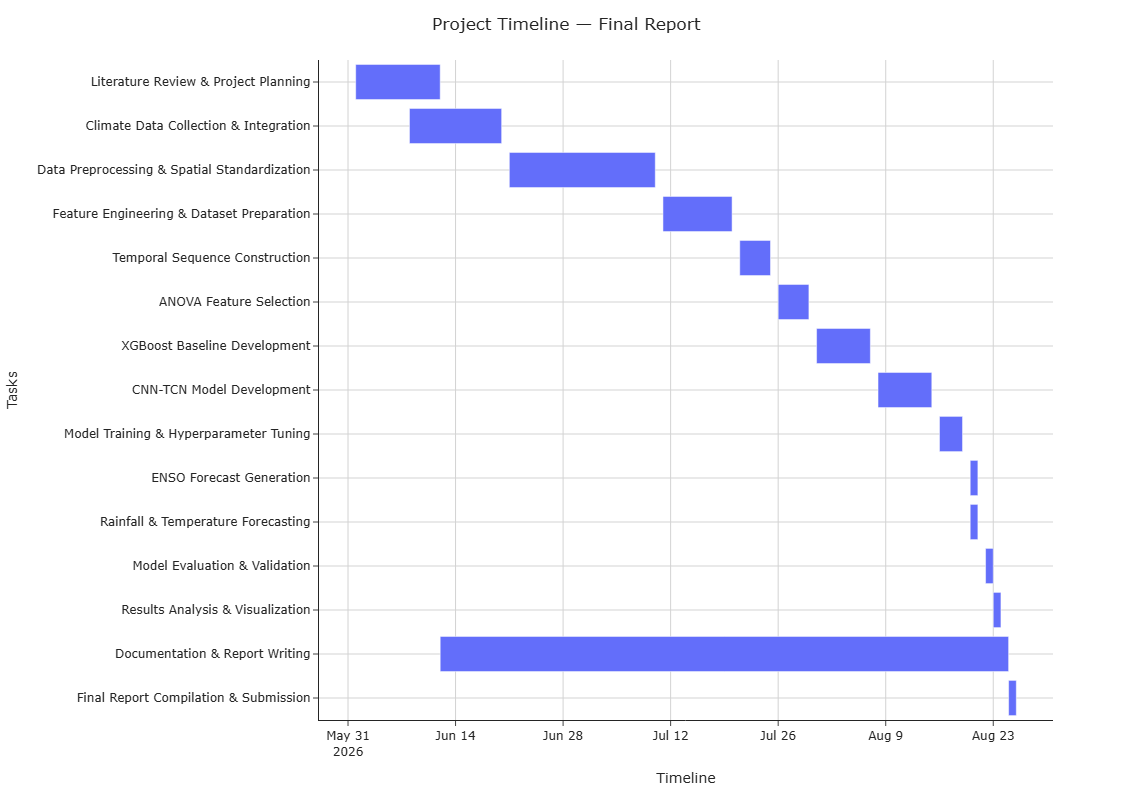
\includegraphics[width=\textwidth]{src/images/gantt_chart.png}
\caption{Project Timeline Gantt Chart}
\label{fig:gantt_chart}
\end{figure}

\newpage
\section*{Appendix C: Details of Dataset}
\addcontentsline{toc}{section}{Appendix C: Details of Dataset}

This appendix summarizes the datasets used for ENSO forecasting and South Asian regional climate impact assessment. Full acquisition and preprocessing details are given in Chapter~\ref{chap:implementation}; this appendix collects the source, coverage, resolution, and variable information for reference.

\subsection*{Dataset Overview}
Three datasets were used: two as model inputs (ERA5, ORAS5) and one as an independent validation reference (the NOAA Ni\~{n}o 3.4 index). All three cover the period 1980--2026, with a fixed 1980--2010 climatological baseline used for anomaly computation.

\begin{table}[H]
\centering
\caption{Summary of datasets used in the project}
\label{tab:dataset_summary}
\normalsize
\renewcommand{\arraystretch}{1.3}
\begin{tabularx}{\textwidth}{|>{\raggedright\arraybackslash}p{0.19\textwidth}|>{\raggedright\arraybackslash}p{0.16\textwidth}|>{\raggedright\arraybackslash}p{0.29\textwidth}|>{\raggedright\arraybackslash}X|}
\hline
\textbf{Dataset} & \textbf{Role} & \textbf{Source} & \textbf{Native Resolution} \\
\hline
ERA5 (Pacific) & Model input & Copernicus CDS & 0.25\degree, regridded to 2\degree \\
\hline
ERA5 (South Asia) & Model input & Copernicus CDS & 0.25\degree, regridded to 2\degree \\
\hline
ORAS5 & Model input & Copernicus CDS (ARCO Zarr) & Curvilinear NEMO grid \\
\hline
NOAA Ni\~{n}o 3.4 Index & Validation reference & NOAA Physical Sciences Laboratory & N/A (index only) \\
\hline
\end{tabularx}
\end{table}

\subsection*{ERA5 Reanalysis}
ERA5 is the fifth-generation atmospheric reanalysis produced by the European Centre for Medium-Range Weather Forecasts (ECMWF) and distributed through the Copernicus Climate Data Store (CDS) API. The monthly-mean product is used throughout this project. Two separate spatial extracts were pulled from the same underlying dataset.

\textbf{Pacific Ocean extract:}
\begin{itemize}
    \item \textbf{Purpose:} ENSO driver variables (SST, atmospheric fields).
    \item \textbf{Spatial domain:} 30\degree N to 30\degree S, 120\degree E to 280\degree E (80\degree W).
    \item \textbf{Resolution:} Regridded to 2\degree $\times$ 2\degree at request time via the CDS \texttt{grid} parameter.
    \item \textbf{Variables fetched:} Sea Surface Temperature (SST), 2-meter temperature, mean sea level pressure, zonal and meridional wind stress components, top-of-atmosphere thermal radiation, and the static land-sea mask (\texttt{lsm}).
\end{itemize}

\textbf{South Asia extract:}
\begin{itemize}
    \item \textbf{Purpose:} Regional climate impact assessment (precipitation and temperature response to ENSO).
    \item \textbf{Spatial domain:} 5\degree N to 35\degree N, 65\degree E to 100\degree E, covering the Indian subcontinent, Nepal, Bangladesh, and surrounding areas.
    \item \textbf{Resolution:} 2\degree $\times$ 2\degree, chosen to resolve regional topographic gradients (the Himalayas, the Western Ghats) that influence monsoon dynamics while remaining computationally tractable.
    \item \textbf{Variables fetched:} Precipitation, 2-meter temperature.
\end{itemize}

\subsection*{ORAS5 Ocean Reanalysis}
ORAS5 (Ocean ReAnalysis System 5) is ECMWF's operational ocean reanalysis, providing subsurface ocean variables not available from atmospheric reanalyses. It was accessed via its Analysis-Ready, Cloud-Optimized (ARCO) Zarr store rather than a direct CDS API request.
\begin{itemize}
    \item \textbf{Purpose:} Subsurface ocean memory predictors, principally Ocean Heat Content.
    \item \textbf{Native grid:} Curvilinear NEMO ocean model grid (not a regular latitude-longitude grid).
    \item \textbf{Regridding:} Interpolated to the same 2\degree $\times$ 2\degree regular grid as the ERA5 Pacific extract, using \texttt{xarray}'s \texttt{interp} method with bilinear interpolation.
    \item \textbf{Key variables:} Upper-300m Ocean Heat Content (\texttt{sohtc300}), sea surface height (\texttt{sossheig}), and 20\degree C isotherm depth (\texttt{so20chgt}), used across both feature-selection methodologies.
\end{itemize}

\subsection*{NOAA Ni\~{n}o 3.4 Index}
The official Ni\~{n}o 3.4 index, published by the NOAA Physical Sciences Laboratory, was not used as a model input. It served exclusively as an independent reference to validate the correctness of the computed Ni\~{n}o 3.4 index (area-averaged SST anomaly over 5\degree S--5\degree N, 170\degree W--120\degree W, against the 1980--2010 baseline). The computed and official indices achieved a Pearson correlation coefficient exceeding 0.95, confirming that the spatial subsetting, regridding, missing-value interpolation, and anomaly computation described in Chapter~\ref{chap:implementation} were implemented correctly.

\subsection*{Temporal Coverage and Splits}
All datasets span 1980--2026 at monthly resolution. After constructing 12-month sliding-window sequences (Section~\ref{sec:tensor-construction}), 542 valid samples remained, split strictly chronologically to prevent data leakage:

\begin{table}[H]
\centering
\caption{Chronological data split used across all models}
\label{tab:dataset_split}
\normalsize
\renewcommand{\arraystretch}{1.2}
\begin{tabular}{|l|l|l|}
\hline
\textbf{Split} & \textbf{Period} & \textbf{Samples} \\
\hline
Train & $\leq$ 2018 & 457 \\
\hline
Validation & 2019--2022 & 48 \\
\hline
Test & 2023--2026 & 40 \\
\hline
\end{tabular}
\end{table}

\subsection*{Final Feature Channels}
Of the variables listed above, four anomaly channels were retained in the spatio-temporal input tensor used by the CNN-TCN model and the two MIFS feature-selection methodologies:

\begin{table}[H]
\centering
\caption{Final input channels used in tensor construction}
\label{tab:dataset_channels}
\normalsize
\renewcommand{\arraystretch}{1.2}
\begin{tabular}{|l|l|l|}
\hline
\textbf{Channel} & \textbf{Variable} & \textbf{Source} \\
\hline
\texttt{sst\_anom} & Sea Surface Temperature anomaly & ERA5 \\
\hline
\texttt{msl\_anom} & Mean Sea Level Pressure anomaly & ERA5 \\
\hline
\texttt{avg\_iews\_anom} & Zonal wind stress anomaly & ERA5 \\
\hline
\texttt{sohtc300\_anom} & Upper-300m Ocean Heat Content anomaly & ORAS5 \\
\hline
\end{tabular}
\end{table}

\subsection*{Access and Licensing}
ERA5 and ORAS5 are both distributed by the Copernicus Climate Change Service (C3S) under the Copernicus license, which permits free use, modification, and redistribution with attribution. Access requires a (free) CDS account and API key. The NOAA Ni\~{n}o 3.4 index is publicly available from the NOAA Physical Sciences Laboratory website with no registration required.


% =====================
% REFERENCES
% =====================
\clearpage
\addcontentsline{toc}{chapter}{REFERENCES}

\nocite{*}

\bibliographystyle{IEEEtran}
\bibliography{report/references}

\end{document}